\documentclass{beamer}
\usetheme{metropolis}           % Use metropolis theme
\usepackage{graphicx} % For including images
\usepackage{tikz}     % For positioning and layering
\usepackage{url} % For handling URLs
\usepackage{tcolorbox} % For creating pretty boxes
\usepackage{caption}
\usepackage{subcaption}
\usepackage[backend=biber]{biblatex} %Imports biblatex package
\addbibresource{references.bib} %Import the bibliography file


% Define a custom tcolorbox style for definitions
\tcbset{
		definitionstyle/.style={
				colback=blue!5!white, % Background color
				colframe=blue!75!black, % Border color
				fonttitle=\bfseries, % Bold title
				coltitle=white, % Title color
				boxrule=0.75mm, % Border thickness
				arc=2.5mm, % Rounded corners
				left=2mm, % Left padding
				right=2mm, % Right padding
				top=1mm, % Top padding
				bottom=1mm % Bottom padding
		}
}
\tcbset{
		theoremstyle/.style={
				colback=black!5!white, % Background color
				colframe=black!75!black, % Border color
				fonttitle=\bfseries, % Bold title
				coltitle=white, % Title color
				boxrule=0.75mm, % Border thickness
				arc=2.5mm, % Rounded corners
				left=2mm, % Left padding
				right=2mm, % Right padding
				top=1mm, % Top padding
				bottom=1mm % Bottom padding
		}
}

% for the sources of images: very small footnotes
\newcommand{\sourcefootnote}[1]{\let\thefootnote\relax\footnote{{\tiny Source: \url{#1}}}}

\title{Temporal Graphs}
% \subtitle{Algorithmic Gems for Graphs, Probabilities and Processes}


\date{January 28, 2025}

\author{Daniel Cermann}

\institute{
	\hfill \begin{minipage}{0.3\textwidth}
		\begin{center}
			
\includegraphics[width=60px]{media/hpi_logo.png} \newline
			Hasso Plattner Institute 
		\end{center}
	\end{minipage}
}

\begin{document}

\begin{frame}
	\begin{center}
		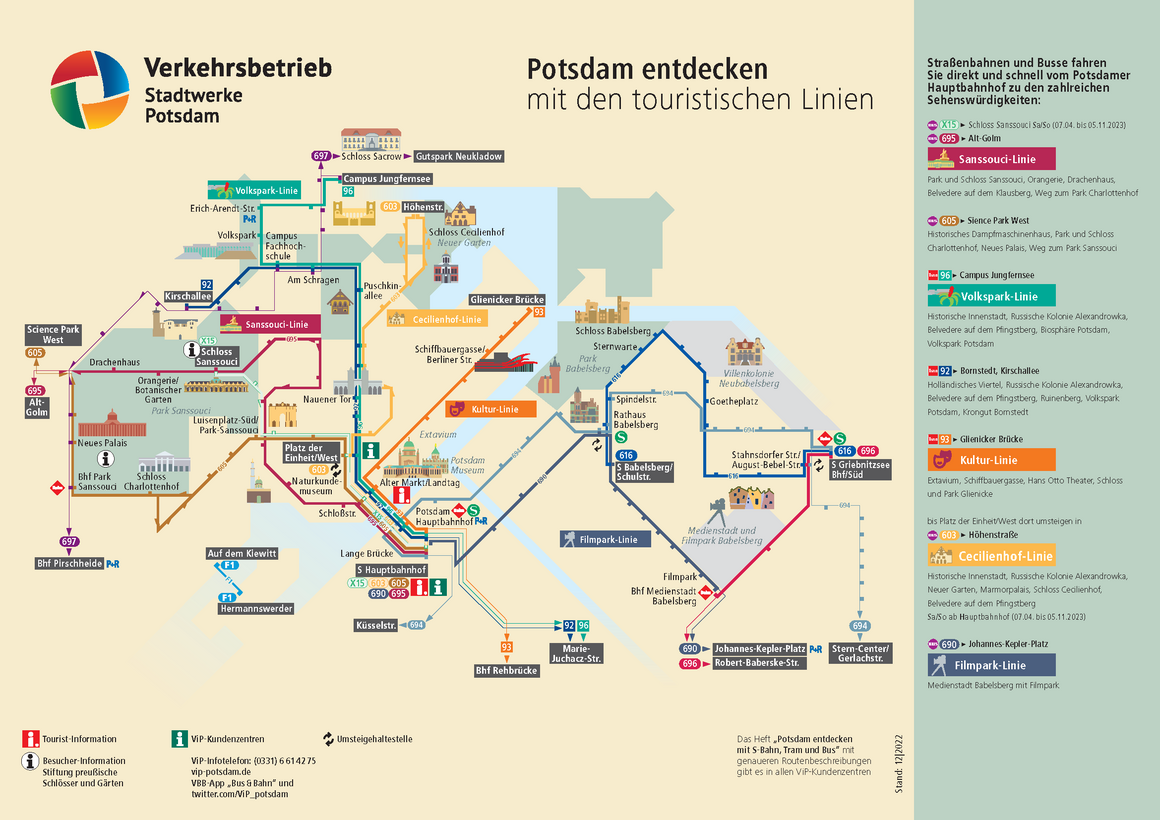
\includegraphics[width=0.95\textwidth]{media/potsdam_citynet.png}
	\end{center}
	\sourcefootnote{https://www.swp-potsdam.de/content/verkehr/bilder_6/liniennetz/touristischer_liniennetzplan_screenshot_1280_960.jpg}
\end{frame}

\maketitle

\section{Motivation}

\begin{frame}{Clip: School day}
	\url{https://youtu.be/BSNJSUkc5-Q?t=996}
\end{frame}

\begin{frame}{Google Maps}
	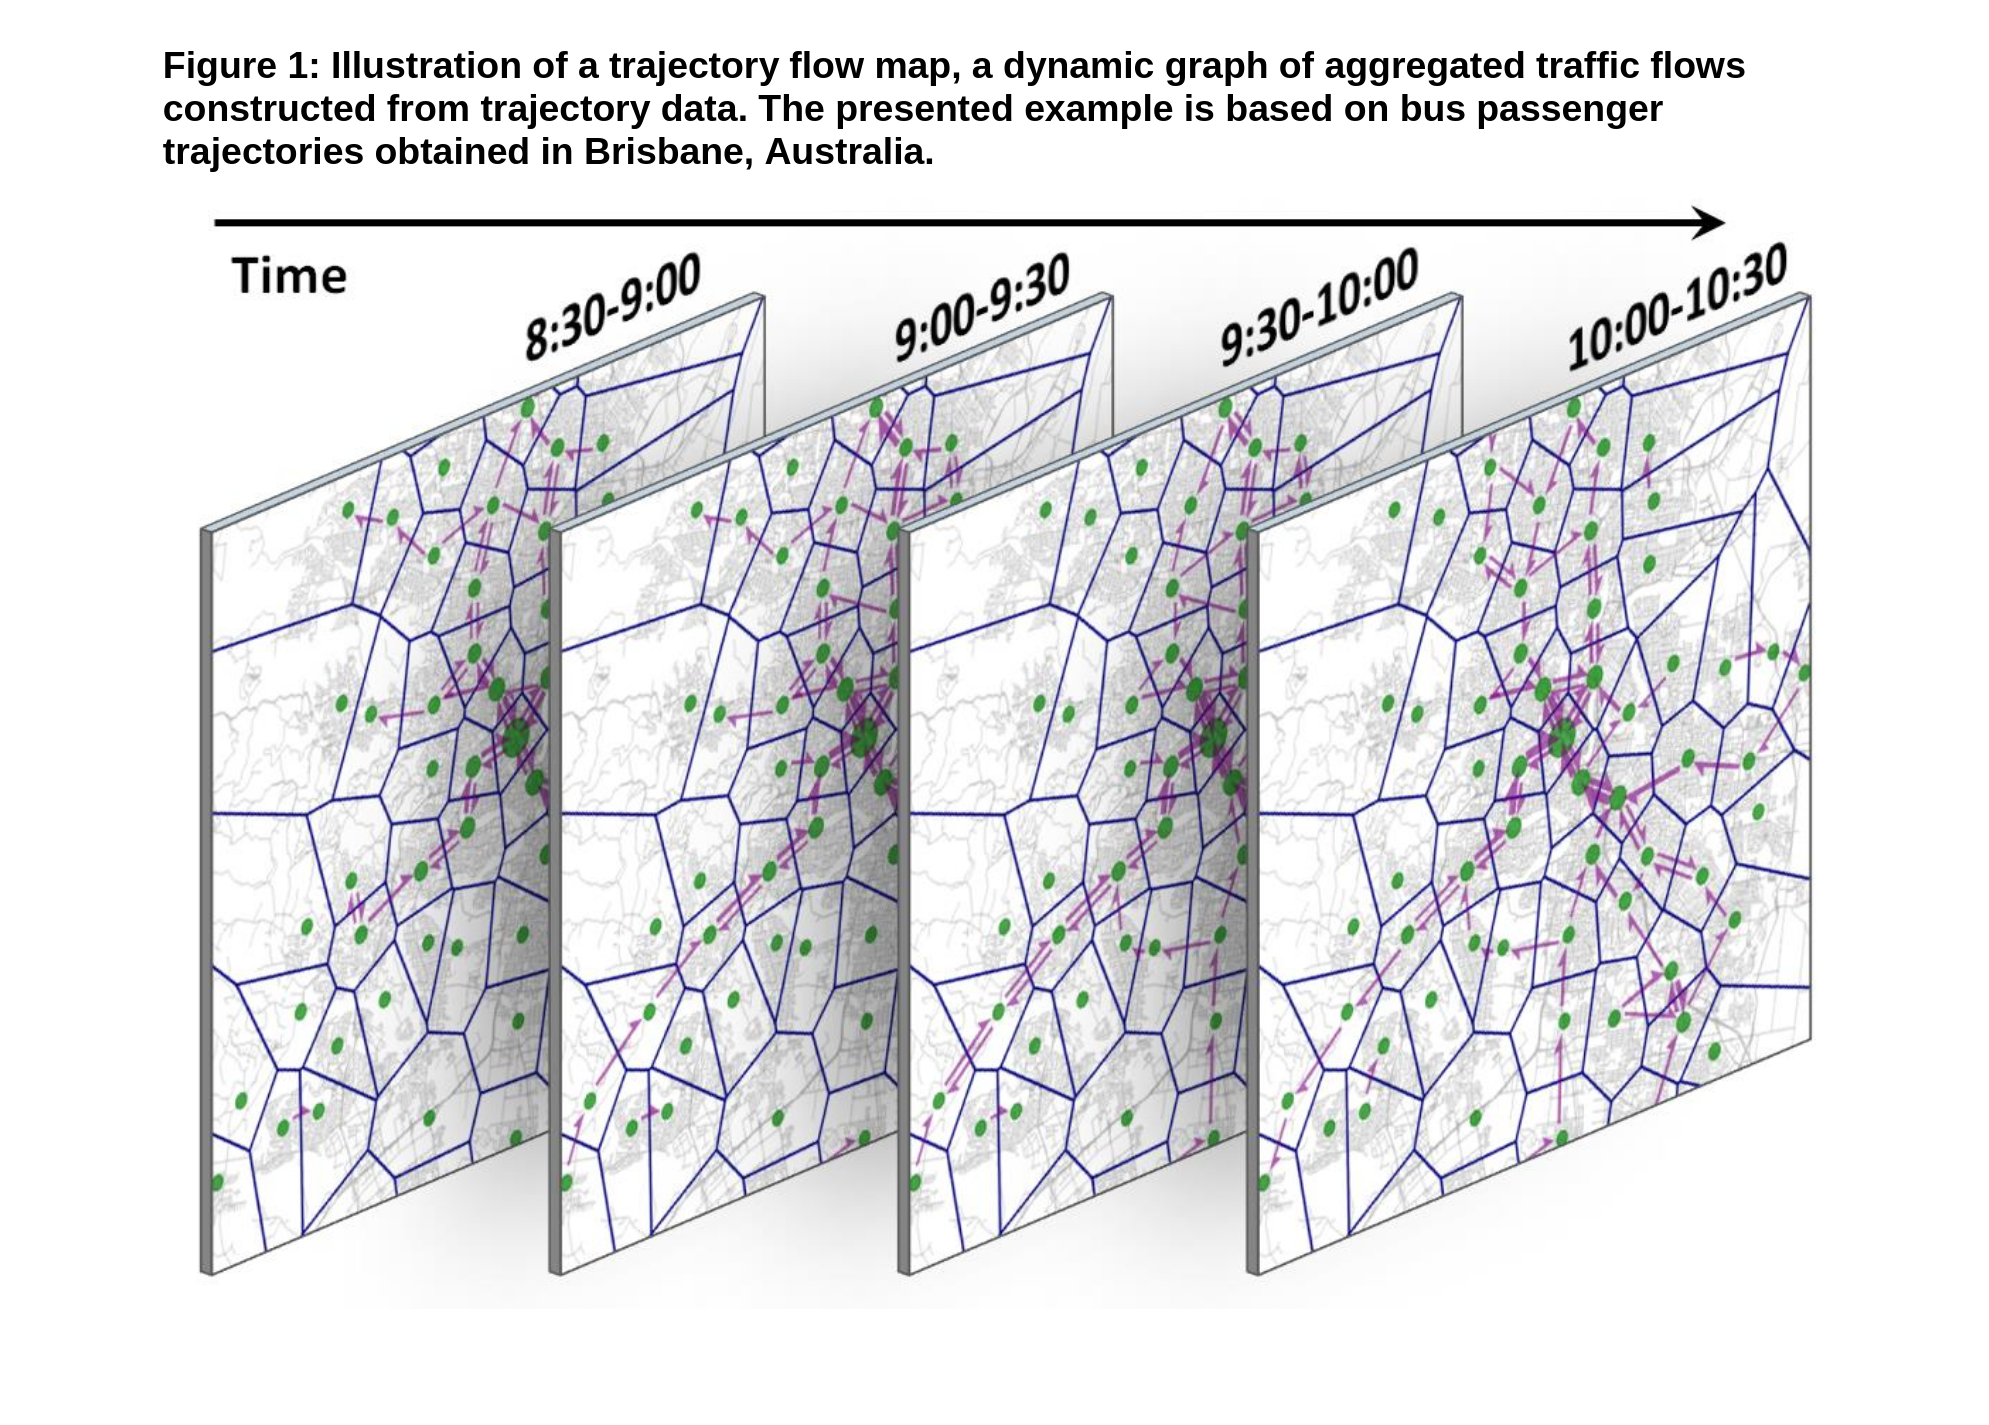
\includegraphics[width=0.9\linewidth]{media/temporal_traffic_data.png} 
	\sourcefootnote{https://australasiantransportresearchforum.org.au/wp-content/uploads/2022/03/ATRF2016_paper_166.pdf}
\end{frame}

\begin{frame}{Distributed systems}
	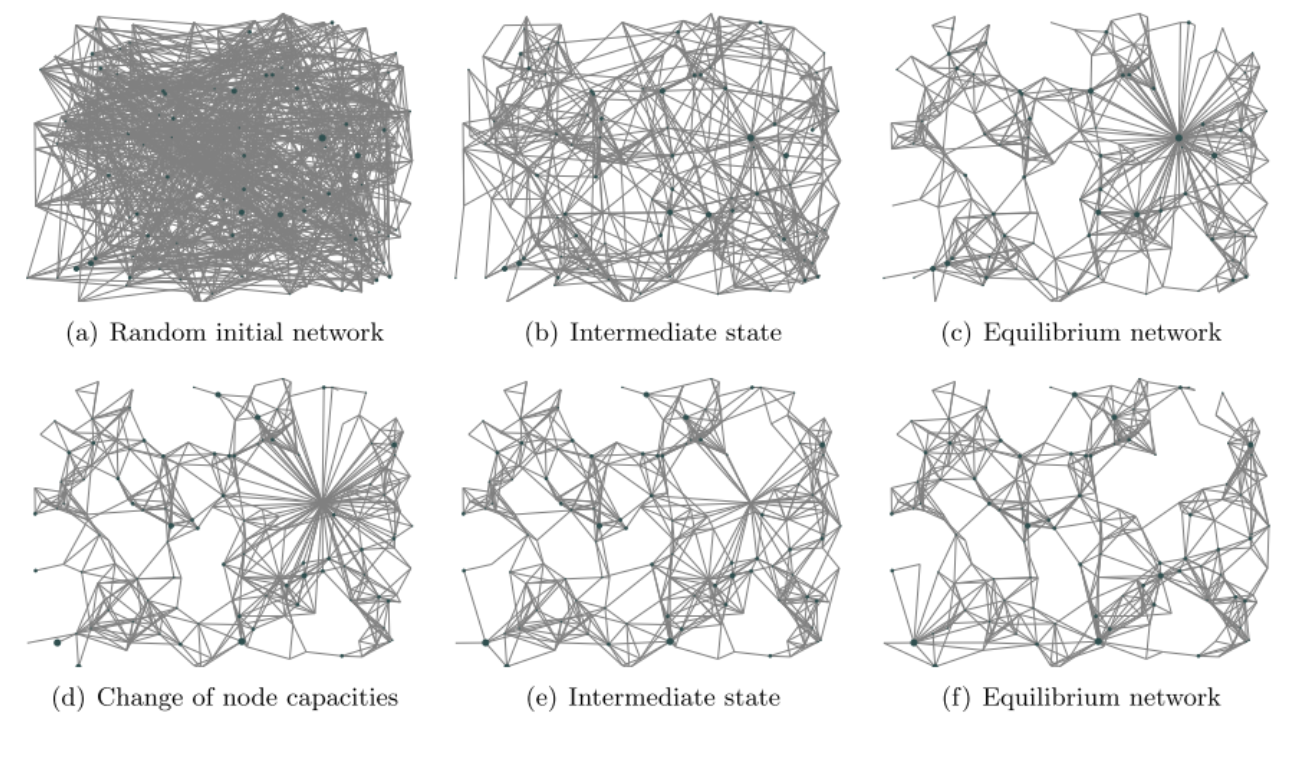
\includegraphics[width=\linewidth]{media/massive_distributed_system.png}
	\sourcefootnote{https://www.sg.ethz.ch/publications/2012/scholtes2012organic-design-of/}
\end{frame}

\begin{frame}{Temporal graphs for physical/chemical models}
	\begin{center}
	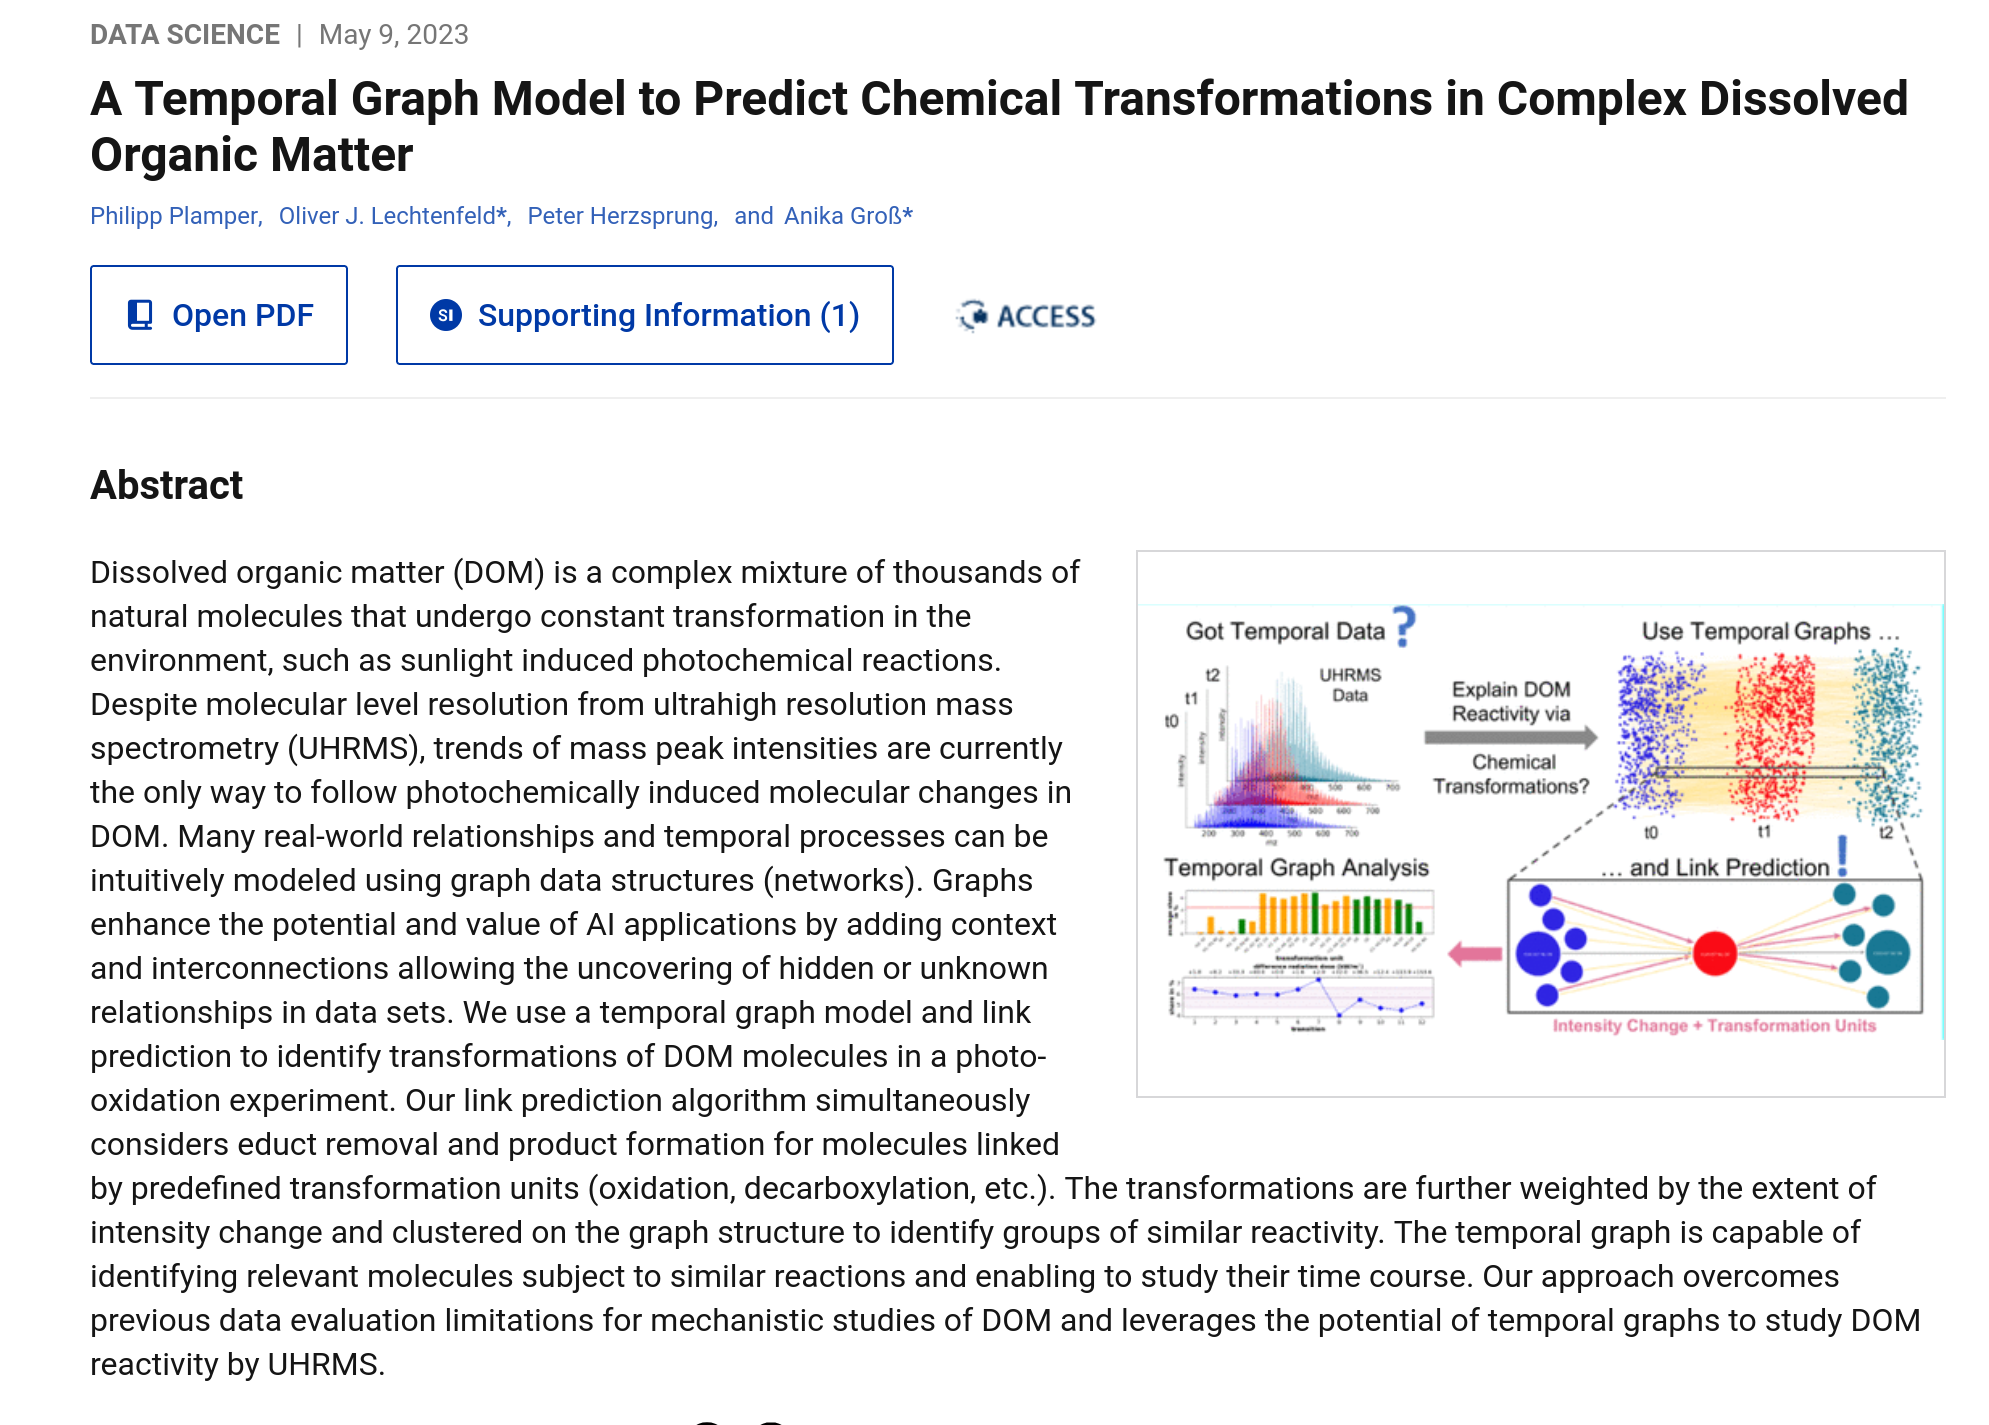
\includegraphics[width=0.8\linewidth]{media/organic_chemistry.png}
	\end{center}
	\sourcefootnote{https://pubs.acs.org/doi/full/10.1021/acs.est.3c00351}
\end{frame}

\begin{frame}{Dissemination processes}
  \centering
  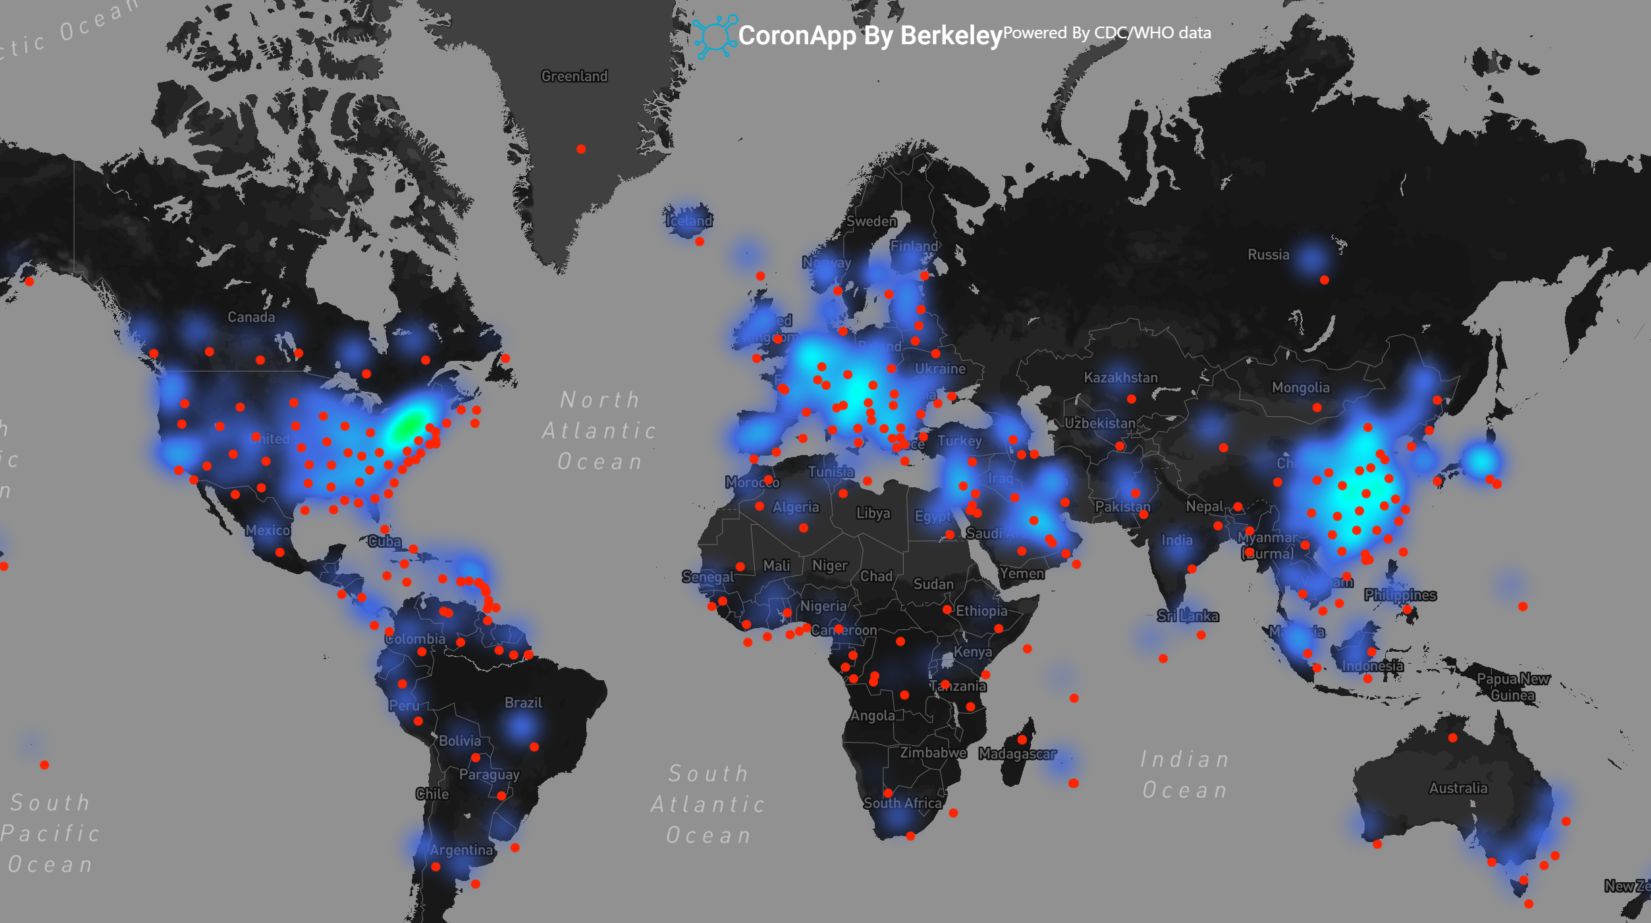
\includegraphics[width=\linewidth]{media/corona.png}
  \sourcefootnote{https://engineering.berkeley.edu/wp-content/uploads/2020/03/CoronApp.png}
\end{frame}


\begin{frame}{How to represent time in graphs?}
		\centering
		\begin{figure}
				\begin{subfigure}{0.42\textwidth}
						\centering
						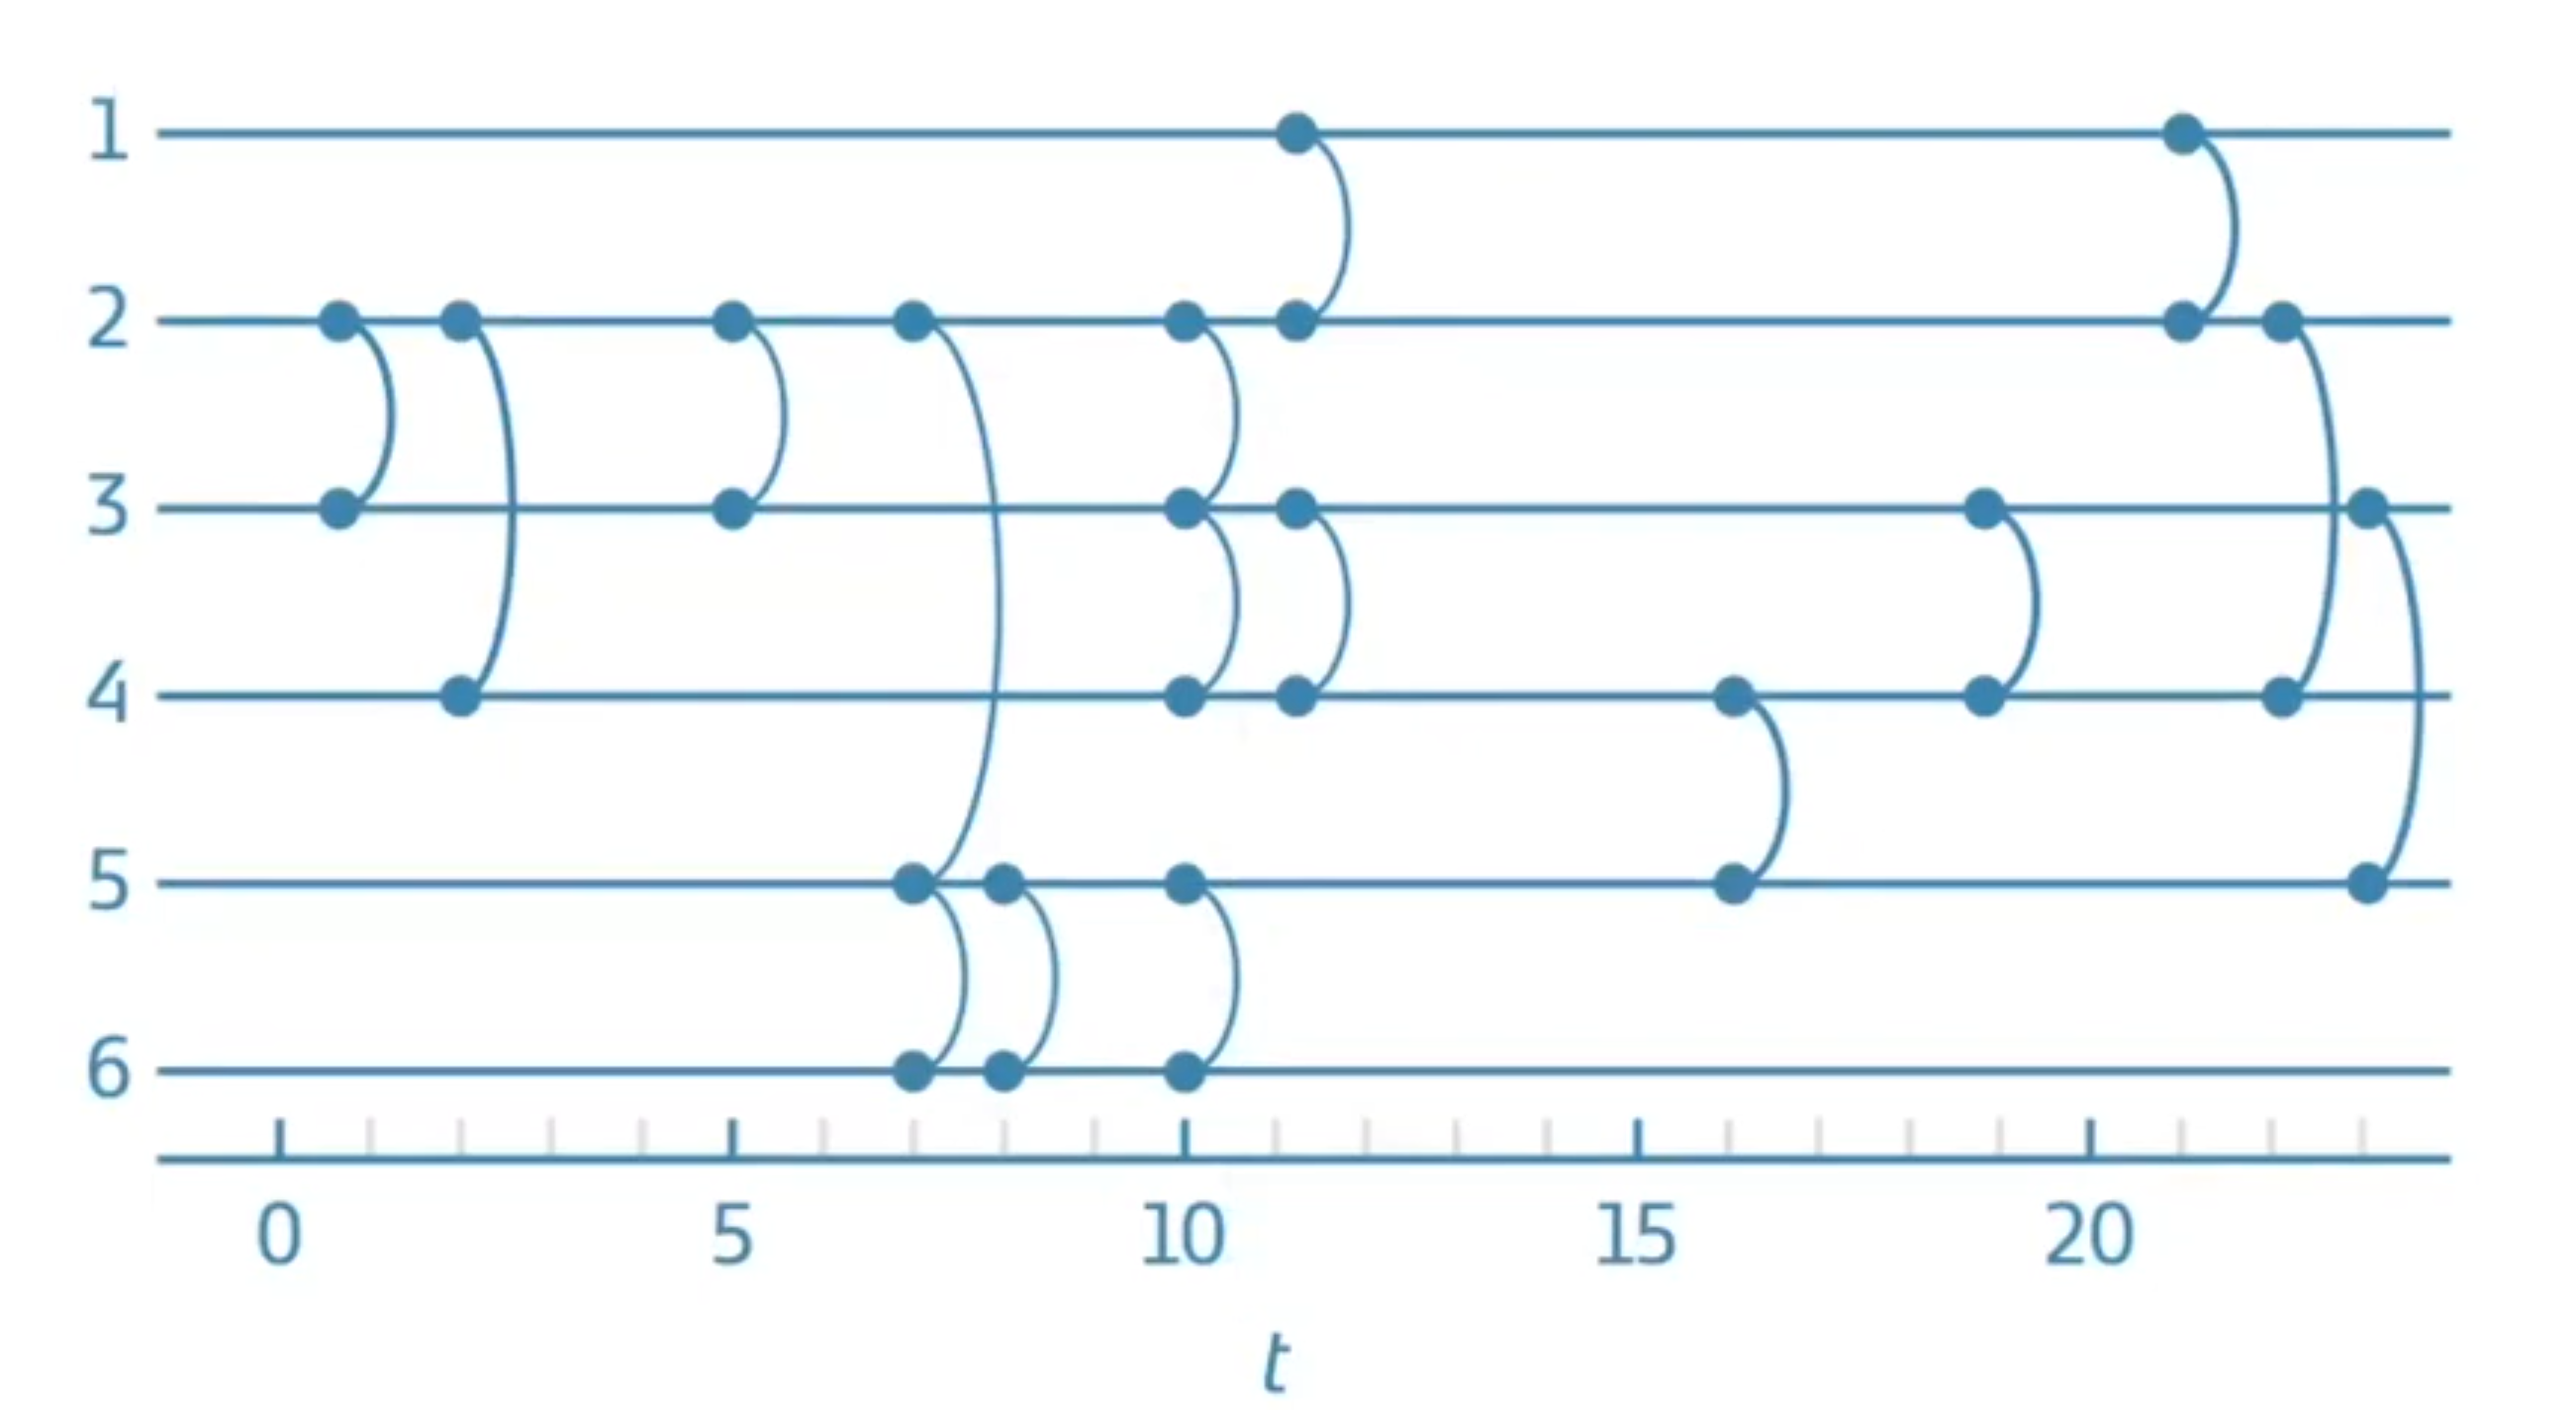
\includegraphics[width=\textwidth]{media/temporal_sense_1.png}
				\end{subfigure}
				\hfill
				\begin{subfigure}{0.42\textwidth}
						\centering
						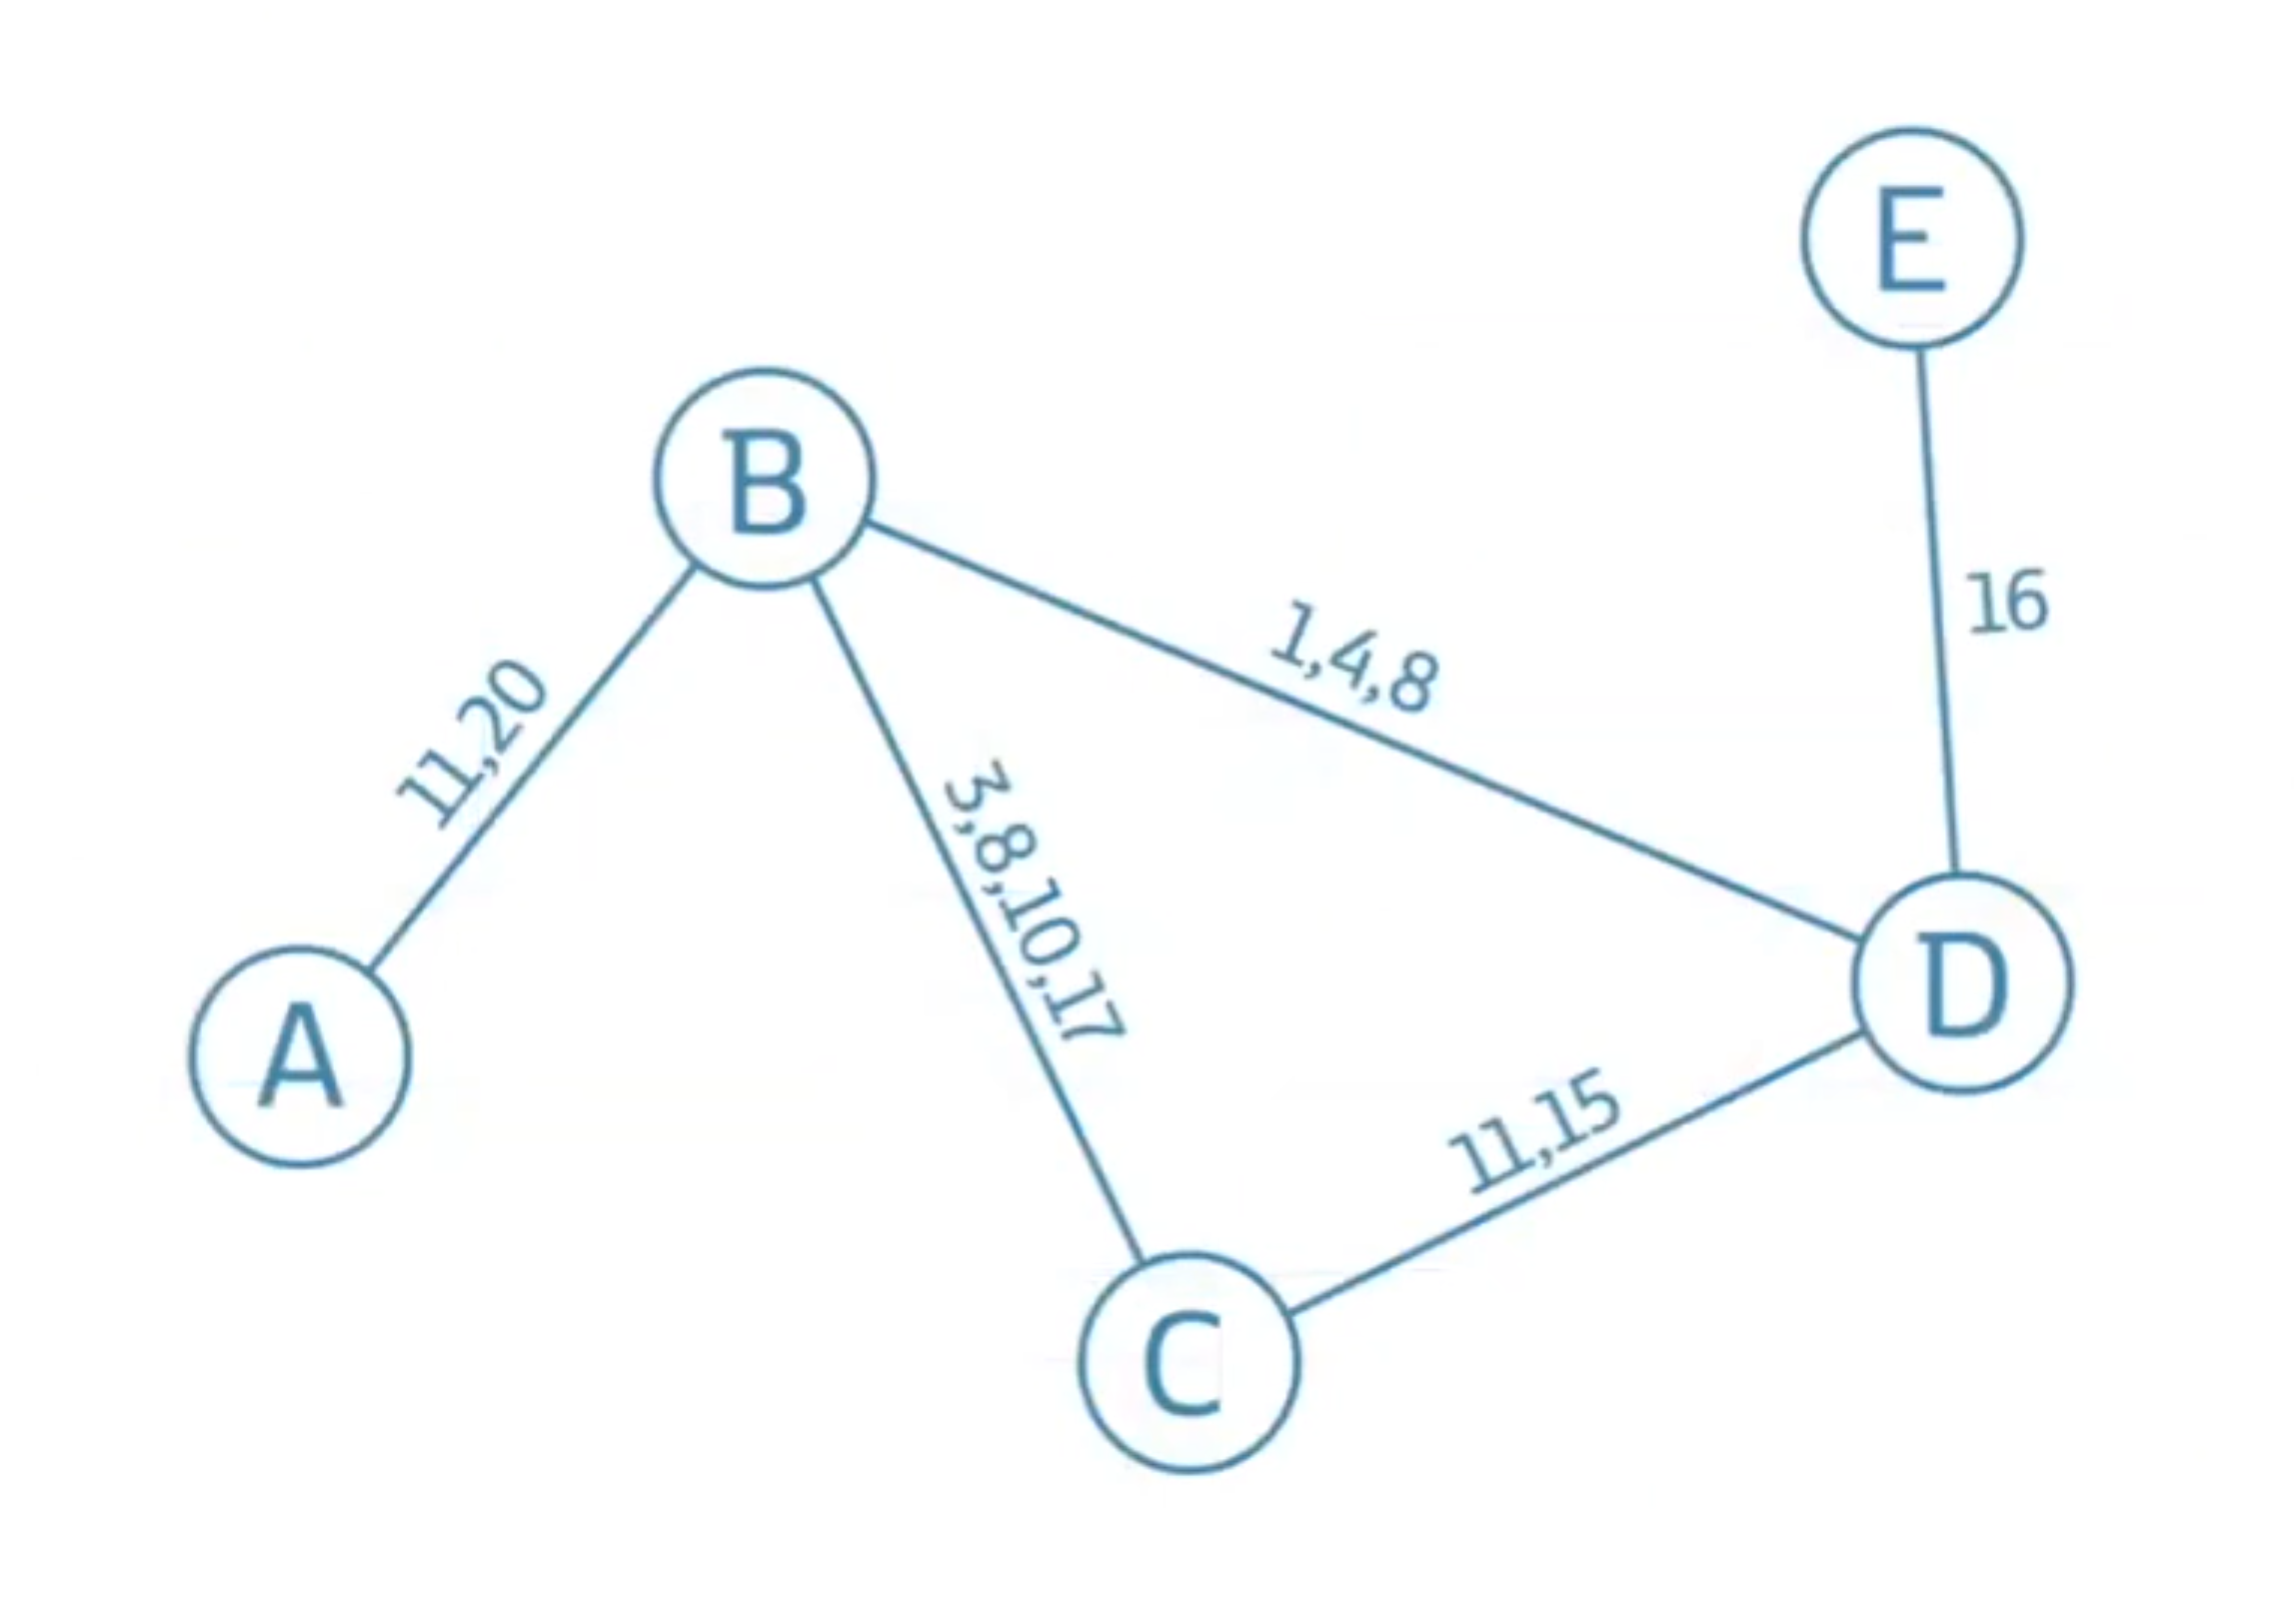
\includegraphics[width=\textwidth]{media/temporal_sense_2.png}
				\end{subfigure}

				\vspace{0.5cm} % Space between rows

				\begin{subfigure}{0.42\textwidth}
						\centering
						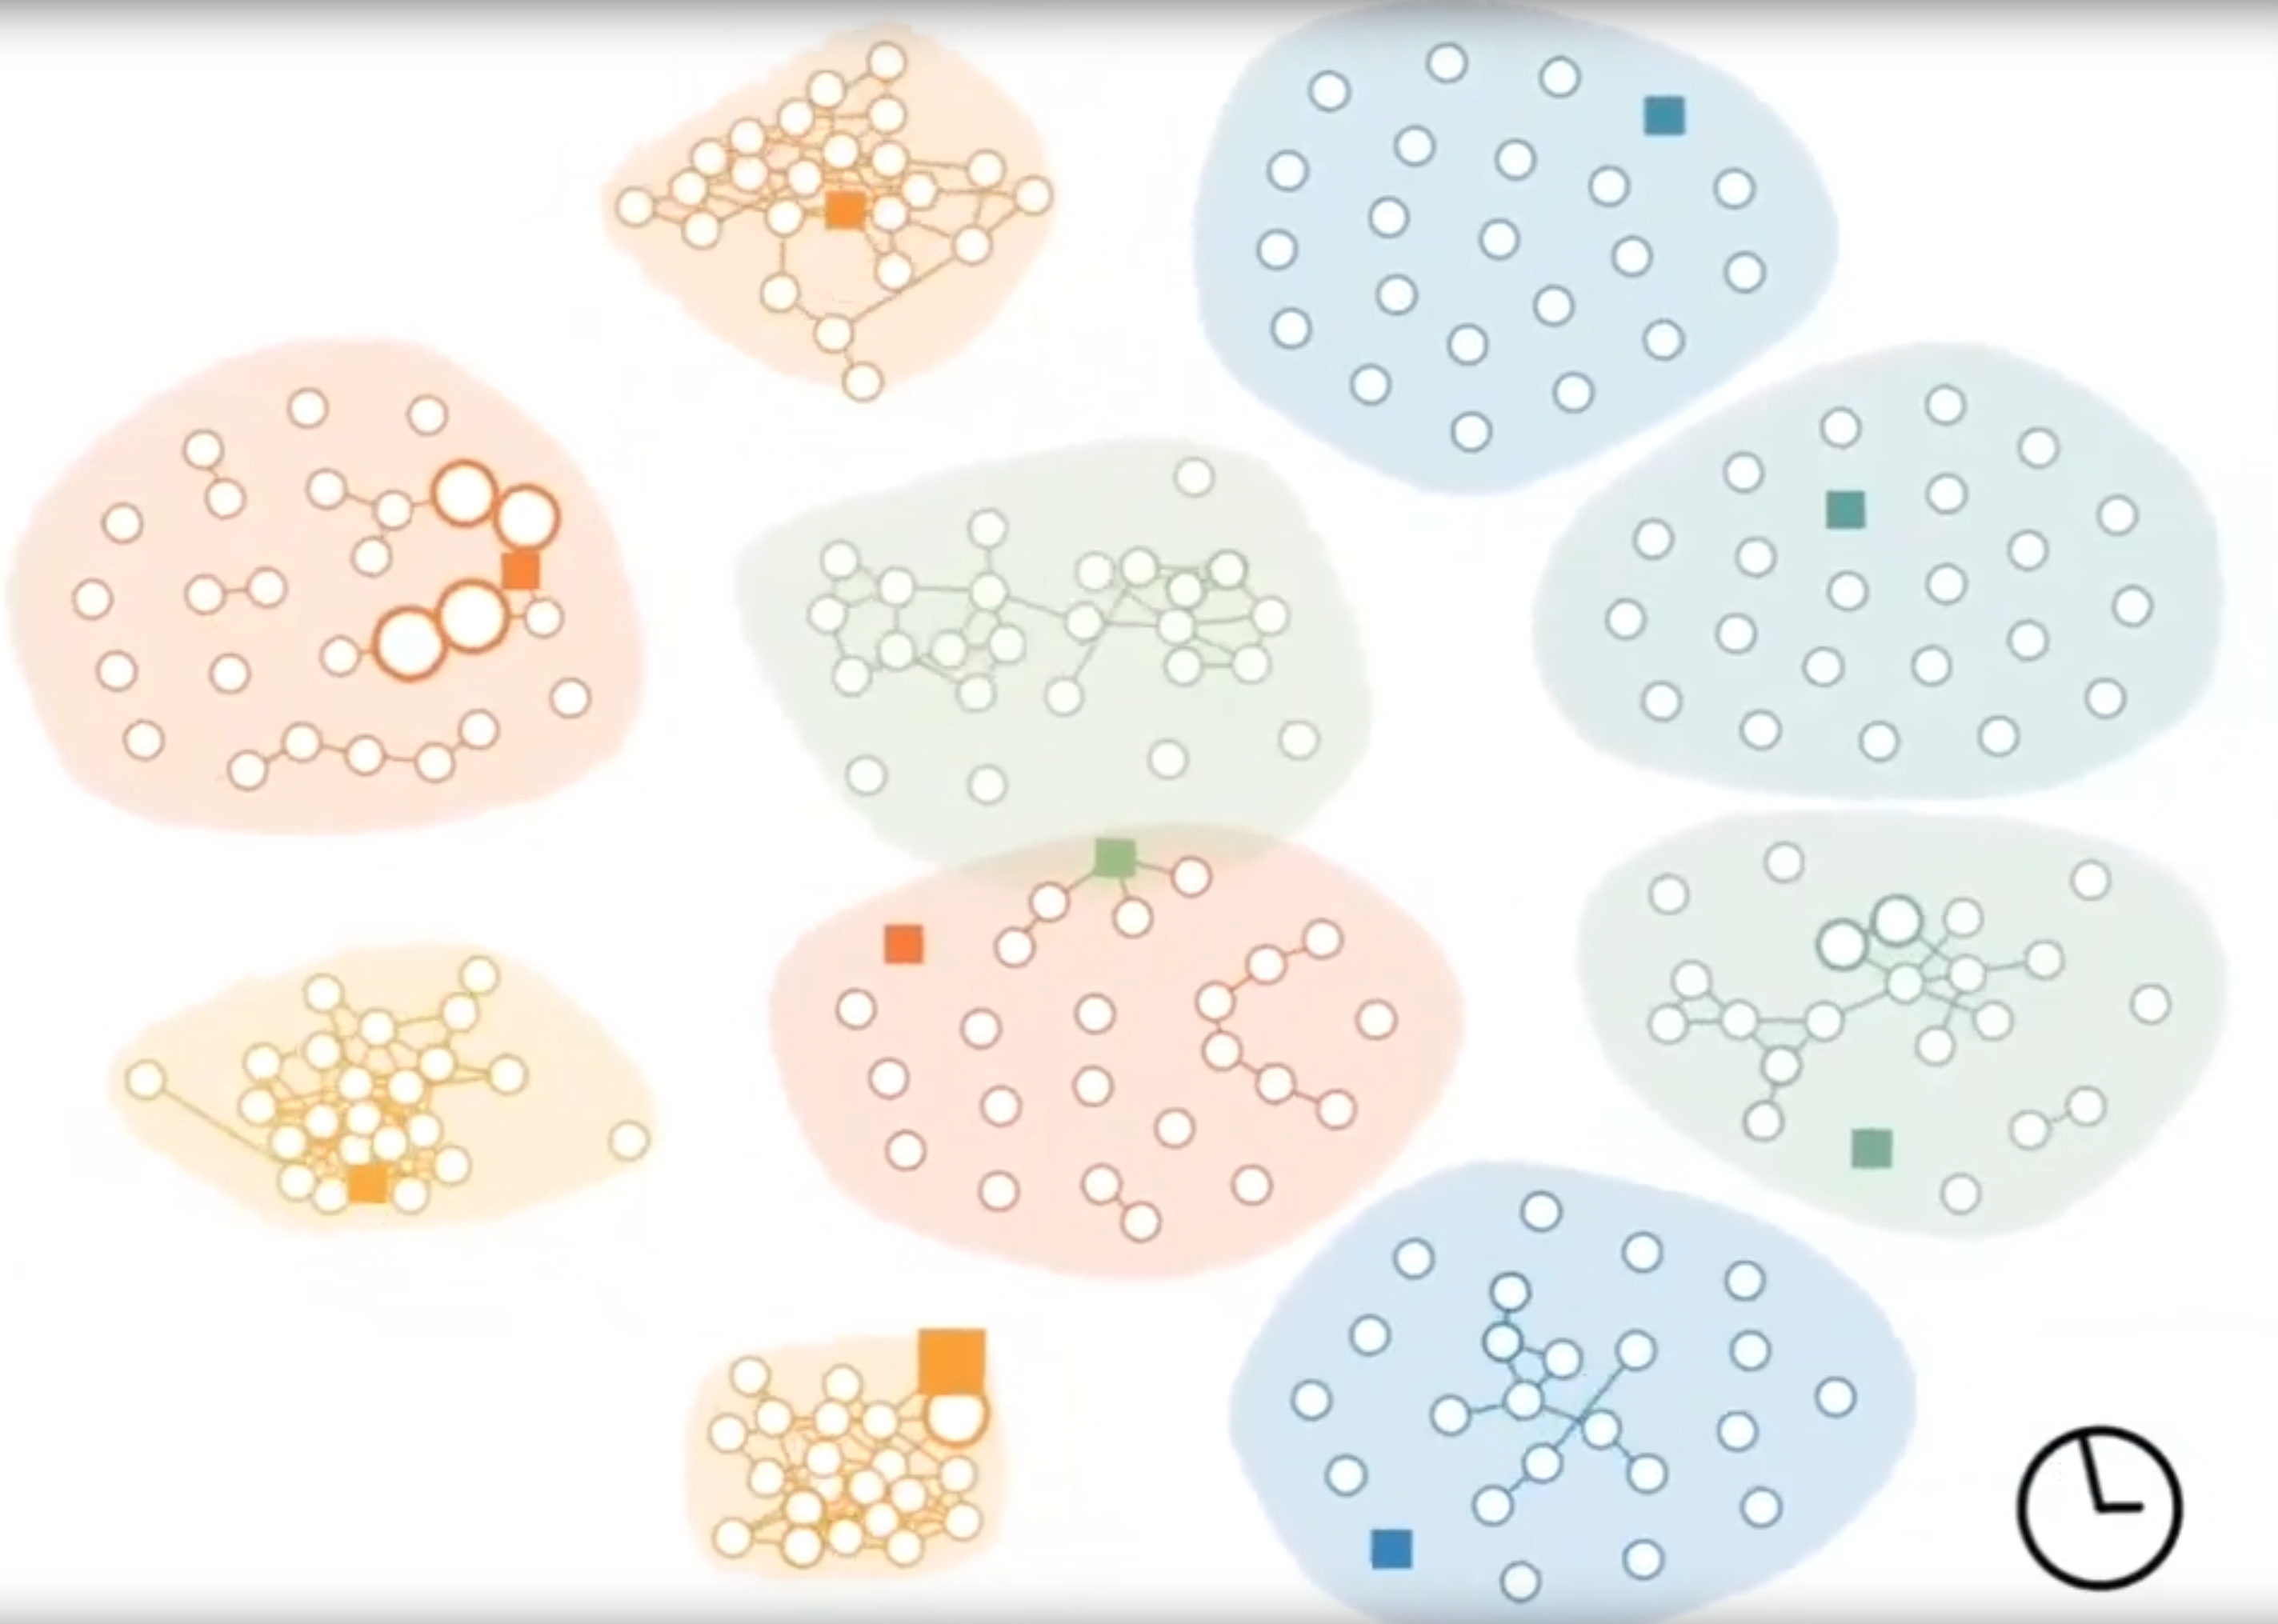
\includegraphics[width=\textwidth]{media/temporal_sense_3.png}
				\end{subfigure}
				\hfill
				\begin{subfigure}{0.42\textwidth}
						\centering
						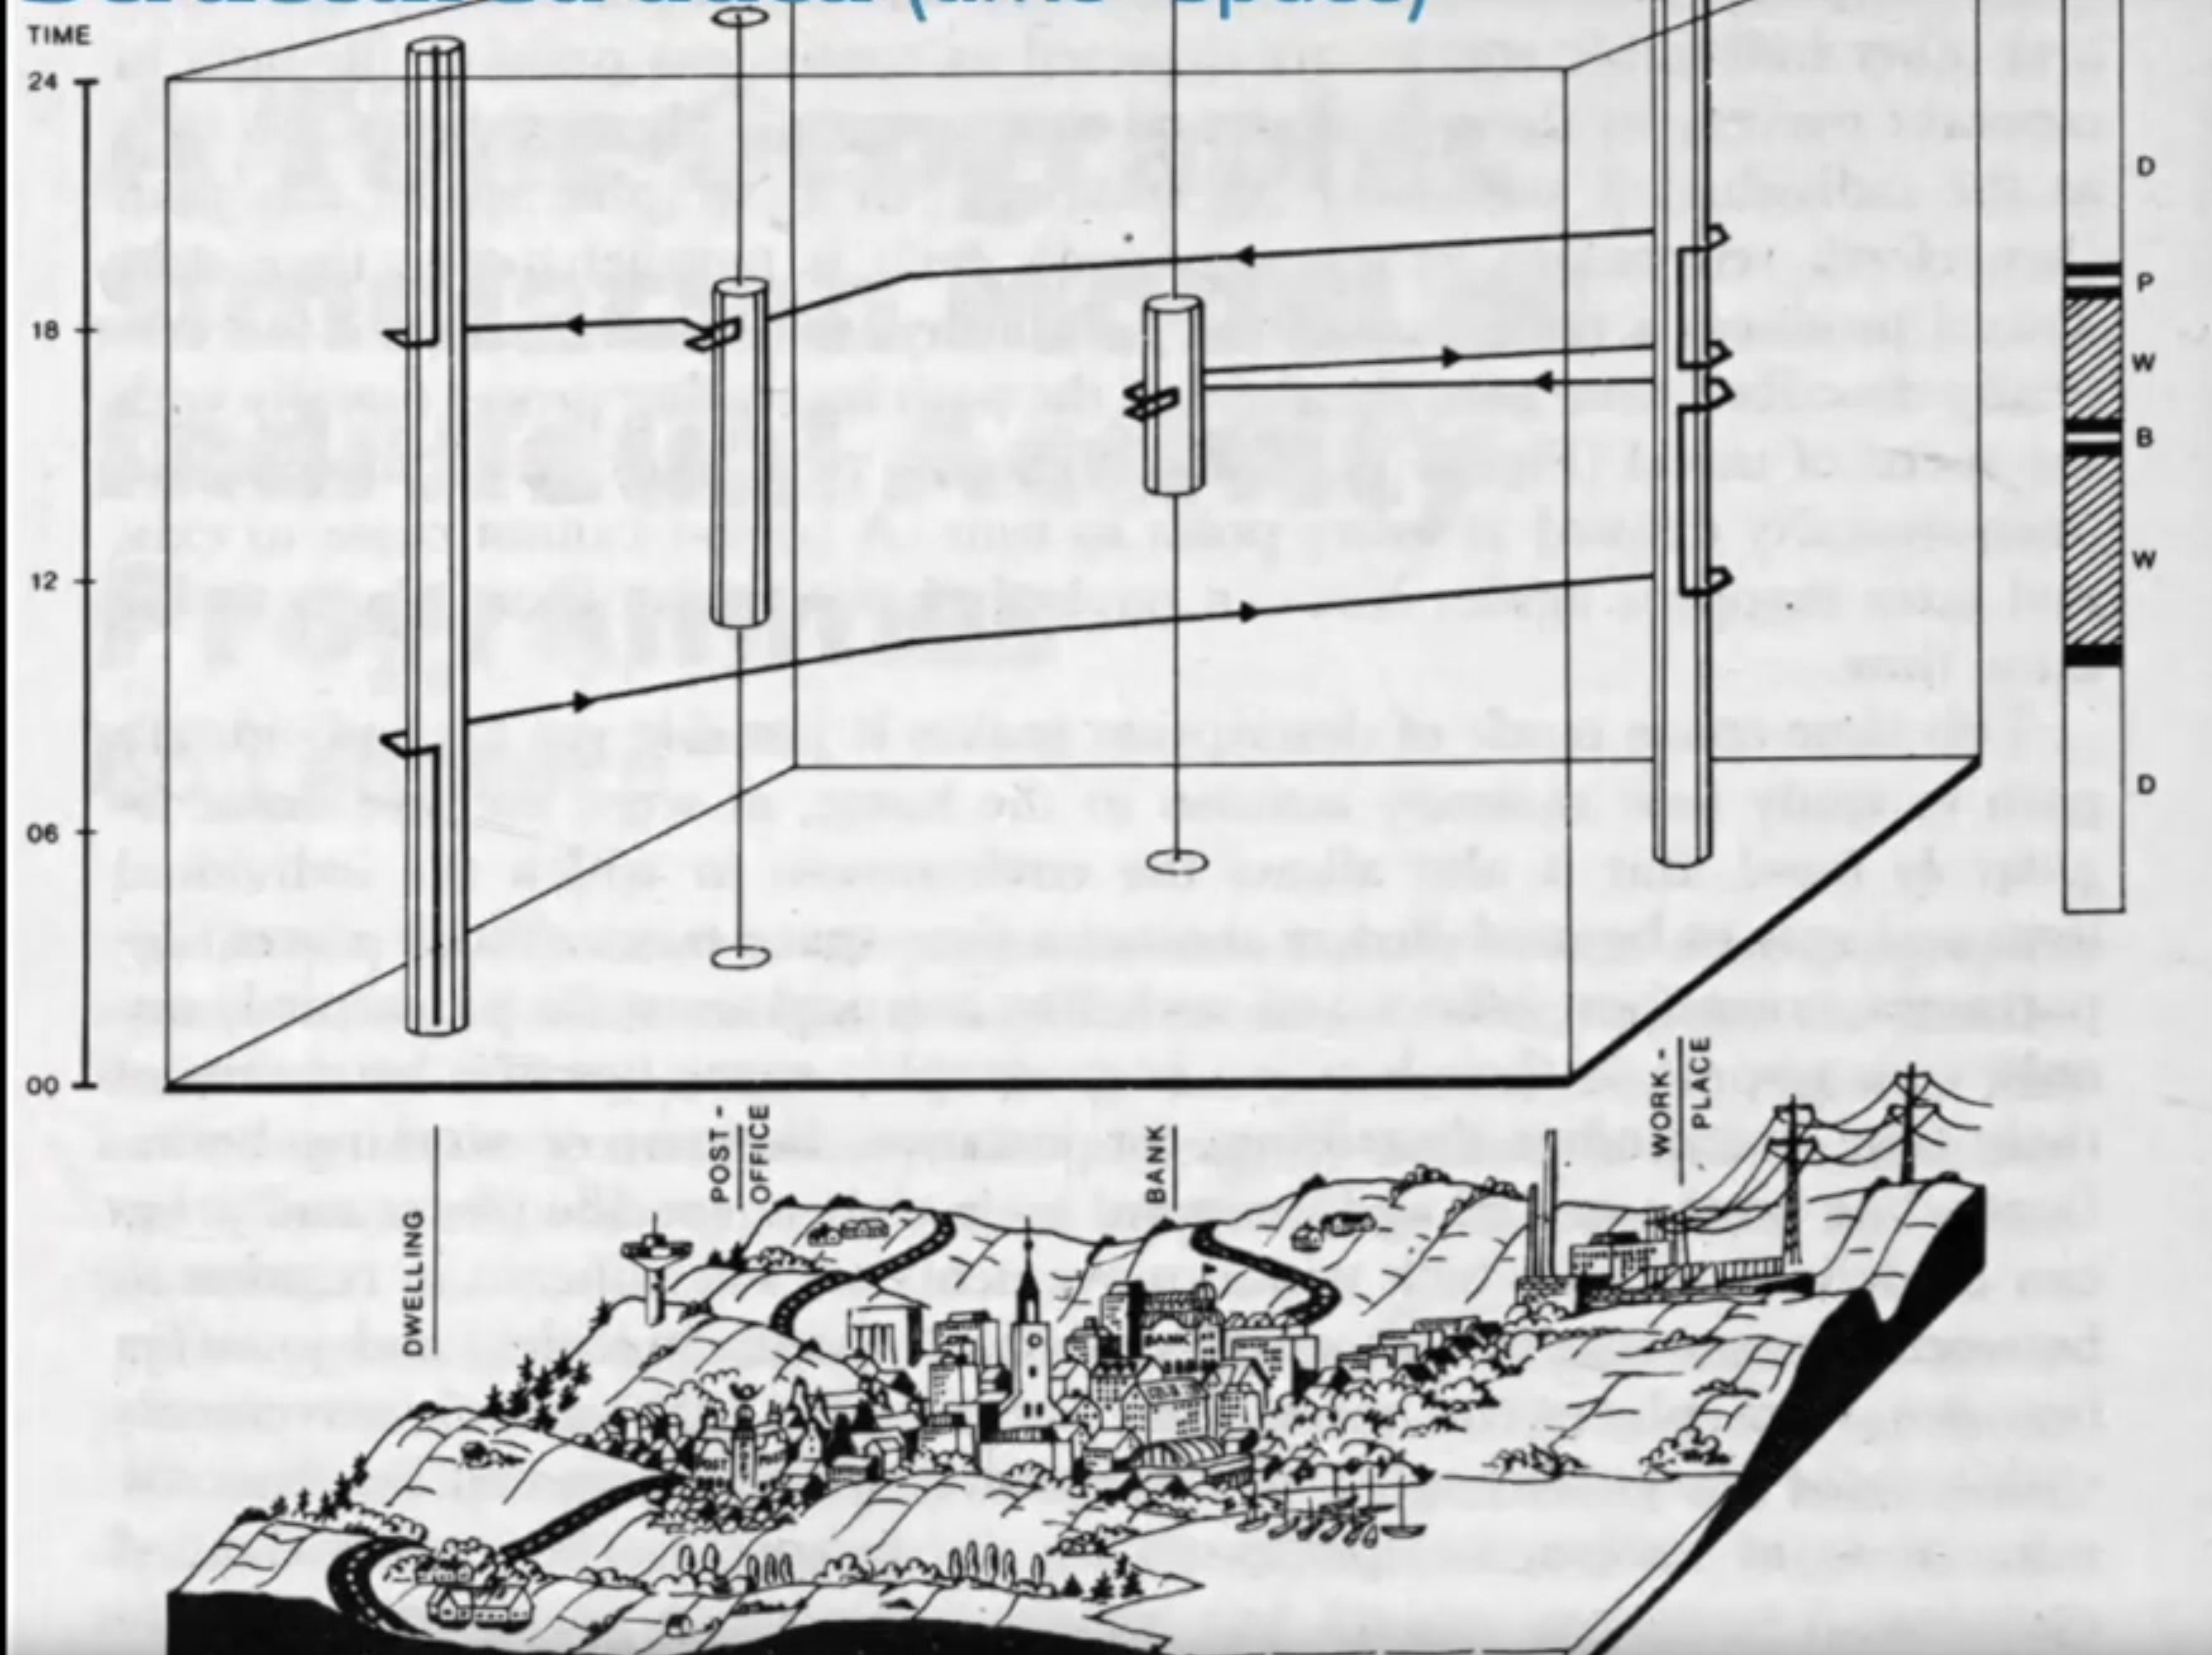
\includegraphics[width=\textwidth]{media/temporal_sense_4.png}
				\end{subfigure}
				\sourcefootnote{https://www.youtube.com/watch?v=BSNJSUkc5-Q}
		\end{figure}
\end{frame}

\section{How to model temporal graphs}
\begin{frame}{How to model temporal graphs}
	\centering
	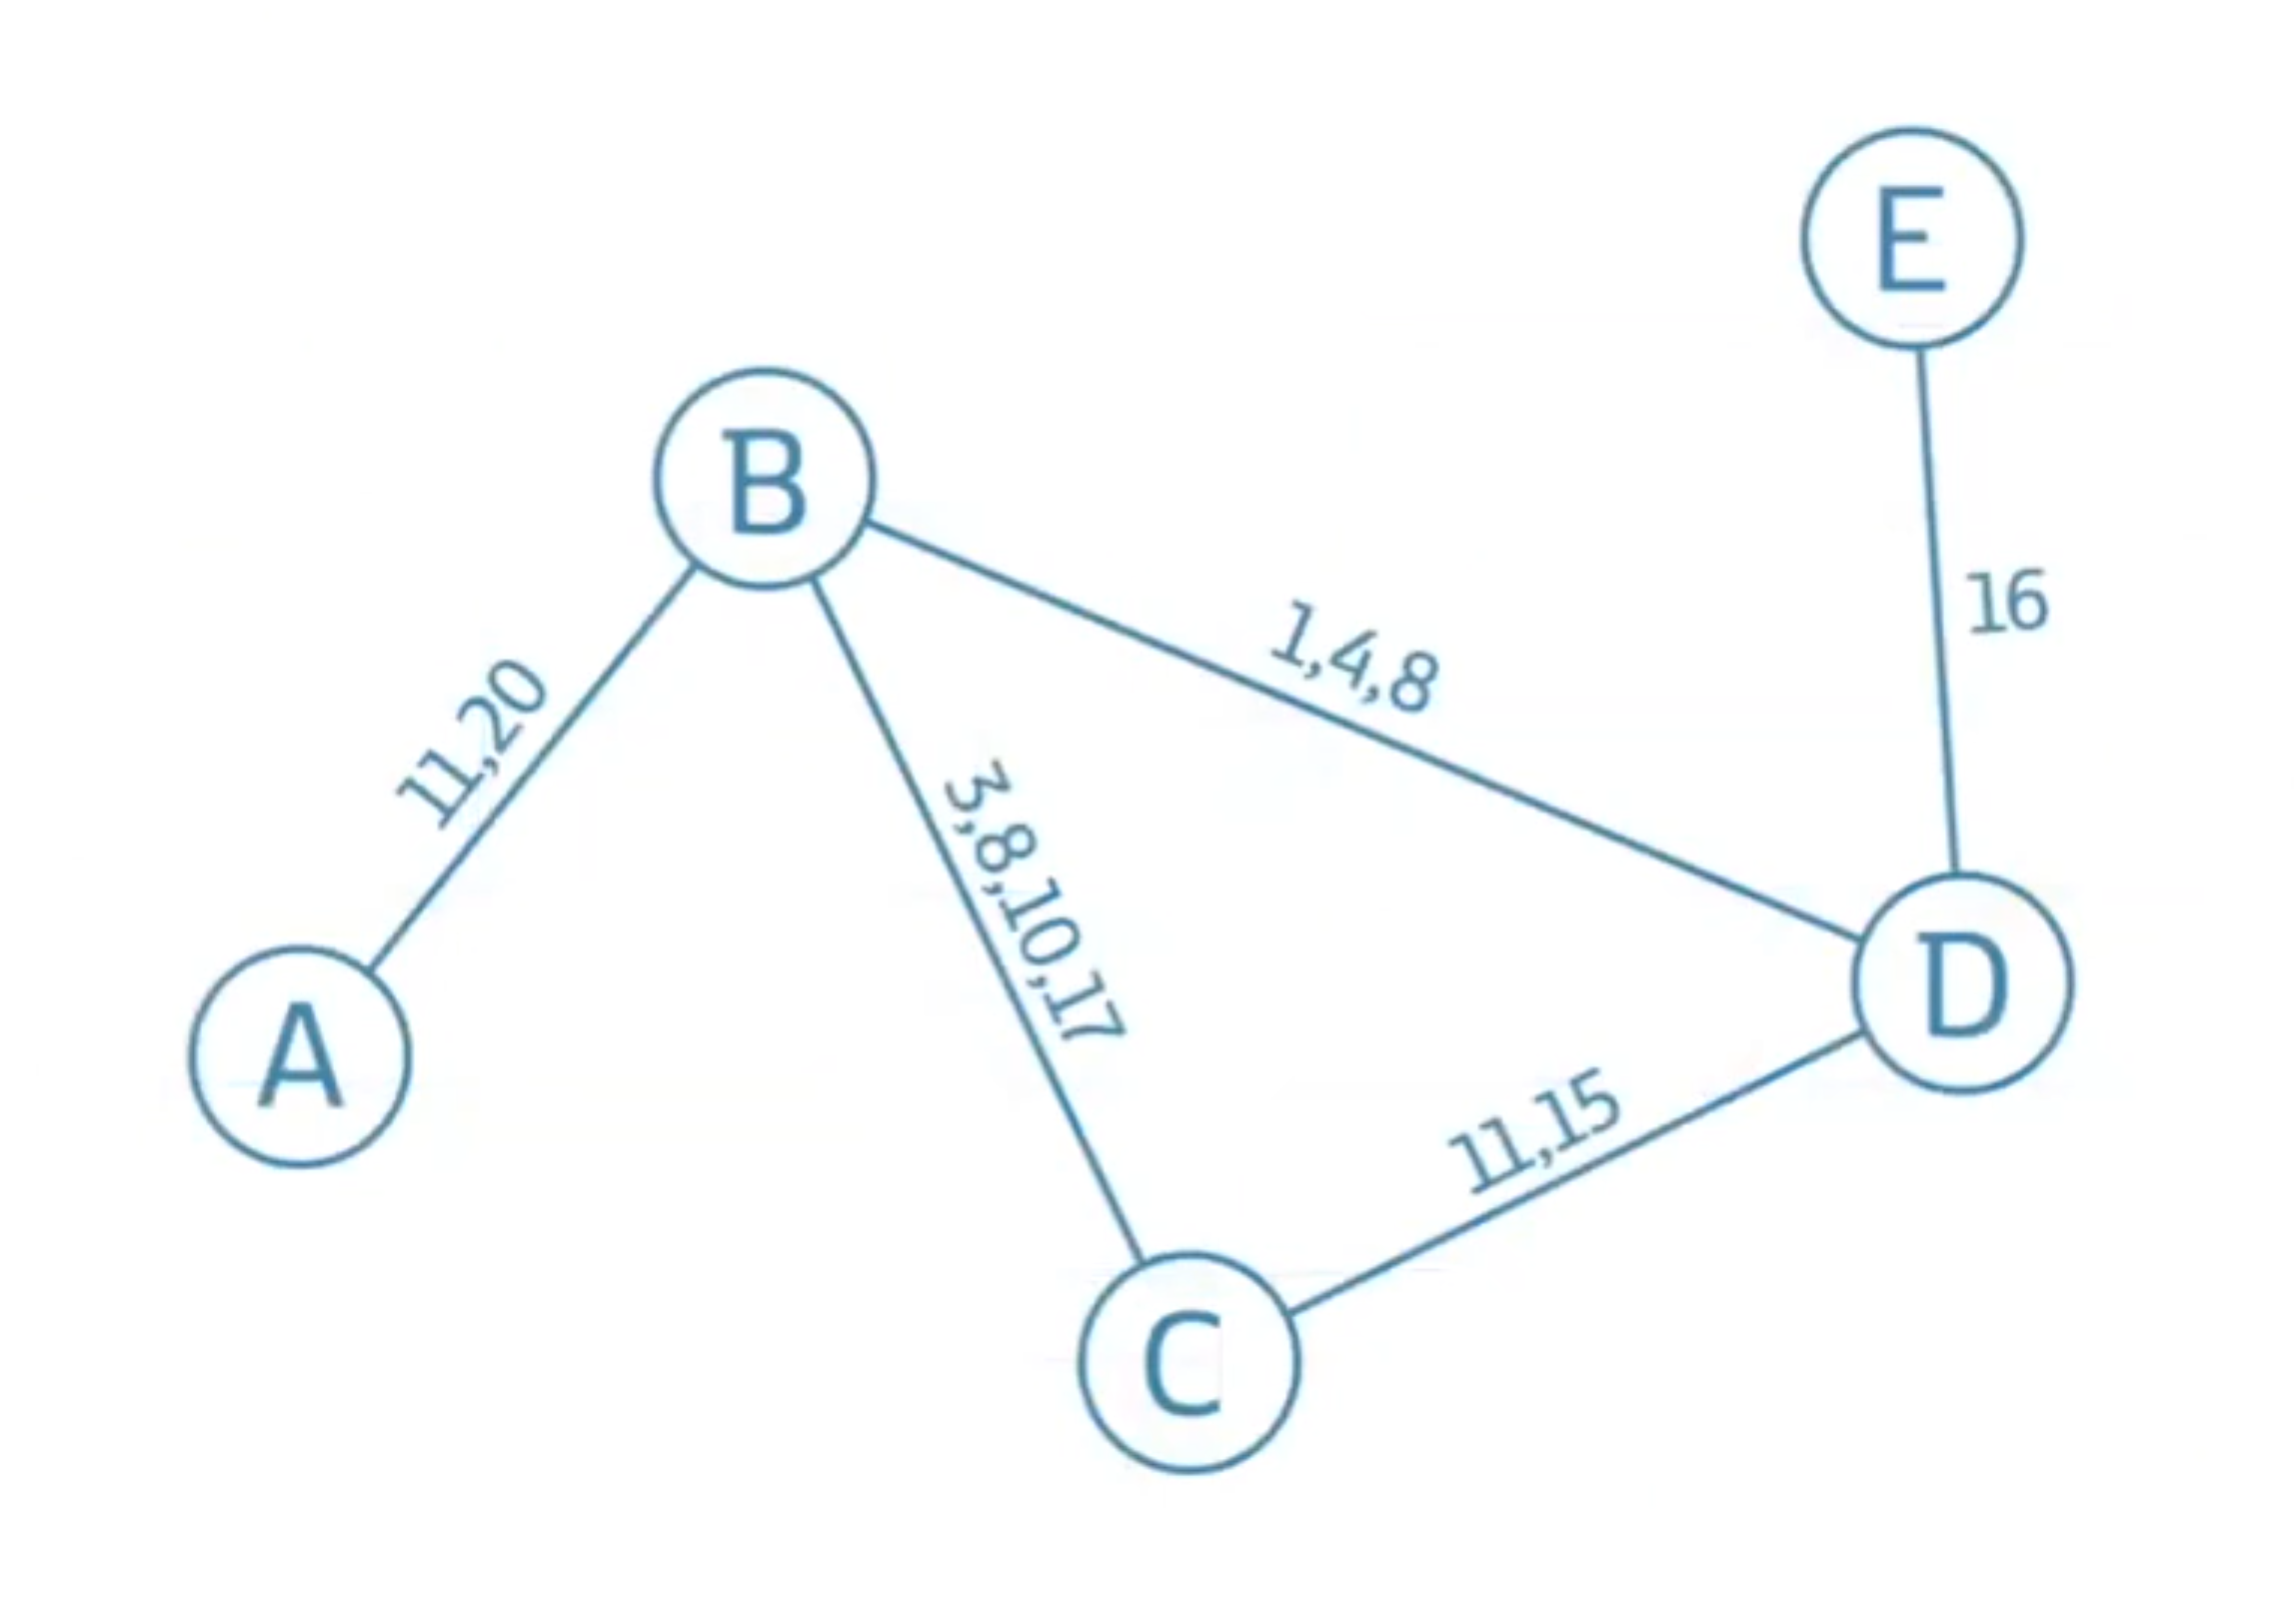
\includegraphics[width=0.9\linewidth]{media/temporal_sense_2.png}
	\sourcefootnote{https://www.youtube.com/watch?v=BSNJSUkc5-Q}
\end{frame}


\begin{frame}{Definition labeled and temporal graphs}
	\visible<1->{
		\begin{tcolorbox}[definitionstyle, title=Definition]
			A \textbf{labeled graph} \cite[page 94]{GHOSH201888} is a triple \( G = (V, E, \lambda) \) where:
				\begin{itemize}
						\item \( V, E \) is a graph
						\item $ \lambda: V \cup E \rightarrow Z$ is a mapping of nodes and edges to a set of labels $Z$
					\end{itemize}
		\end{tcolorbox}
		}

	\visible<2->{
	 \begin{tcolorbox}[definitionstyle, title=Definition]
			A \textbf{temporal graph} \cite[page 243]{Michail2015} is is triple \( G = (V, E, \lambda) \) where:
			\begin{itemize}
						\item \( V, E \) is a graph
						\item $ \lambda: E \rightarrow 2^{\mathbb{N}}$ is a mapping edges to a set natural numbers (time steps when this edge is active)
					\end{itemize}
		\end{tcolorbox}
	}
\end{frame}

\begin{frame}{Relationship labeled and temporal graphs}
  \begin{minipage}{0.45\textwidth}
    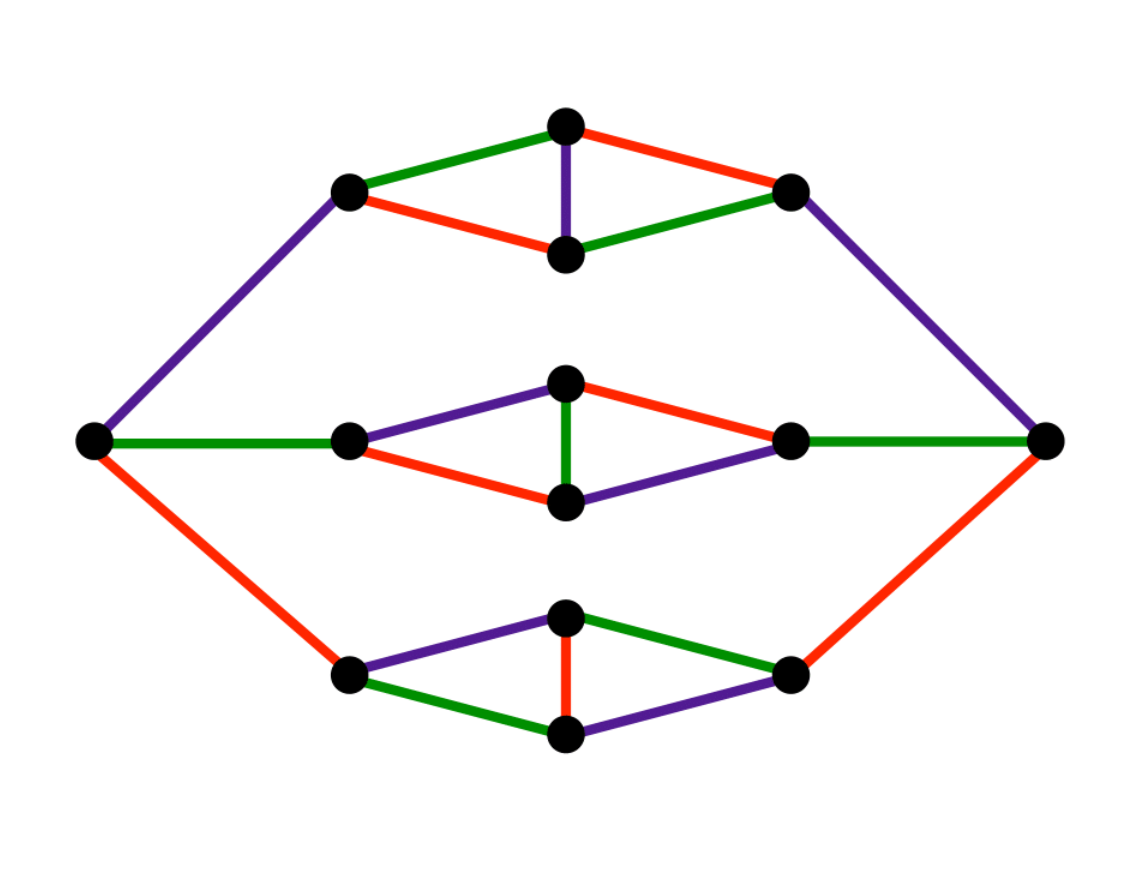
\includegraphics[width=\linewidth]{media/proper_edge_coloring.png}
    \sourcefootnote{https://www.algorist.com/images/figures/edge-coloring-R.png}
  \end{minipage}
  \hfill $\leftrightarrow$ \hfill
  \begin{minipage}{0.45\textwidth}
  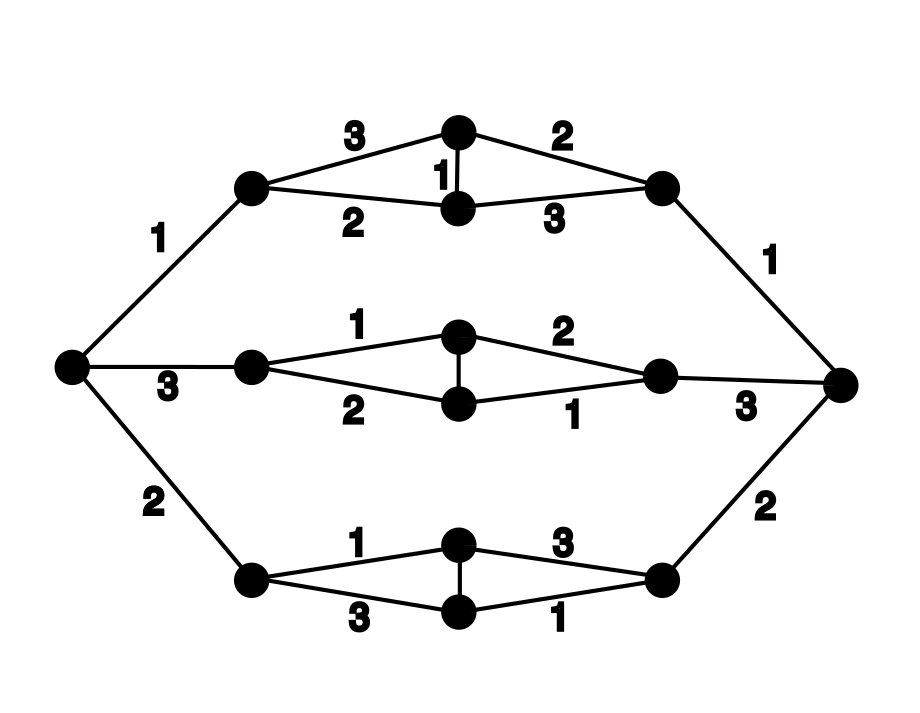
\includegraphics[width=\linewidth]{media/edge_coloring_to_temporal_graph.png}
  \sourcefootnote{me :)}
  \end{minipage}
\end{frame}

\begin{frame}{Notation for convenience $\rightarrow$ \cite[p. 243ff]{Michail2015}}
\begin{itemize}
	\item $\lambda(G)$ - temporal graph with respect to $G$
	\item $\lambda(E)$ - multiset of all labels
	\item $| \lambda | = \sum_{e \in E} | \lambda(e) | $
	\item $ \lambda_{min} = min\{l \in \lambda(E)\} $
	\item $ \lambda_{max} = max\{l \in \lambda(E)\} $
	\item $\alpha(\lambda) = \lambda_{max} - \lambda_{min} + 1$ - lifetime of a temporal graph $\lambda(G)$
\end{itemize}
\end{frame}

\begin{frame}{Transitivity of reachability in static graphs}
		\begin{tcolorbox}[theoremstyle, title=Reachability in a static graph is transitive]
      Given A static graph $G = (V, E)$, for all nodes $A, B, C \in V$ we have:
      If B is reachable by A and C is reachable by B, then C is reachable by A. \\
      \begin{center}
      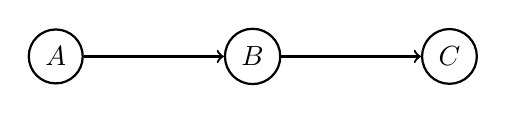
\begin{tikzpicture}[->, node distance=2.5cm, thick, main/.style = {draw, circle}]
        % Nodes
        \node[main] (A) {$A$};
        \node[main] (B) [right of=A] {$B$};
        \node[main] (C) [right of=B] {$C$};
        % Edges
        \draw (A) -- (B);
        \draw (B) -- (C);
     \end{tikzpicture}
     \end{center}
		\end{tcolorbox}
\end{frame}

\begin{frame}{Transitivity of reachability in static graphs}
  \begin{center}
    \large
    Is reachability in a temporal graph transitive?
  \end{center}
\end{frame}

\begin{frame}{Time matters!}
  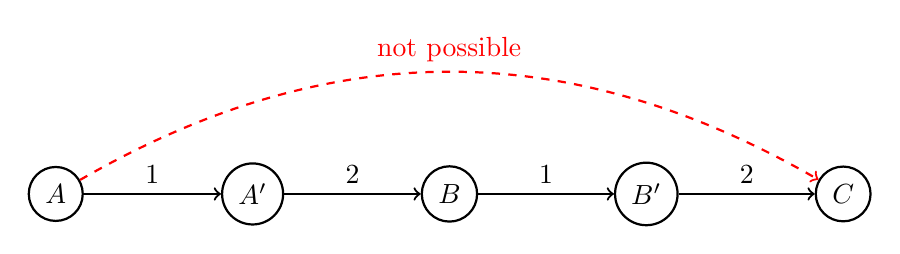
\begin{tikzpicture}[->, node distance=2.5cm, thick, main/.style = {draw, circle}]
    % Nodes
    \node[main] (A) {$A$};
    \node[main] (A_prime) [right of=A] {$A'$};
    \node[main] (B) [right of=A_prime] {$B$};
    \node[main] (B_prime) [right of=B] {$B'$};
    \node[main] (C) [right of=B_prime] {$C$};

    % Edges with time labels
    \draw (A) -- (A_prime) node[midway, above] {1};
    \draw (A_prime) -- (B) node[midway, above] {2};
    \draw (B) -- (B_prime) node[midway, above] {1};
    \draw (B_prime) -- (C) node[midway, above] {2};

    % Crossed-out edge to show non-reachability
    \draw[red, dashed] (A) edge[bend left] node[midway, above] {not possible} (C);
  \end{tikzpicture} \\[5ex]
  $\Longrightarrow$ Deep implications for complexity of temporal graphs
\end{frame}

\begin{frame}{Notation \#2}
\begin{itemize}
	\item A temporal graph $D$ is an ordered set of disjoint sets $(V, A)$
	\item $A \subseteq V^2 \times \mathbb{N}$ - 'time edges'
	\item $A(t) = \{e | (e, t) \in A\}$ - set of edges at time $t$
	\item $D(t) = (V, A(t))$ - snapshot of graph D at time $t$
\end{itemize}
\end{frame}

\begin{frame}{Static expansion of a temporal graph}
	\begin{center}
		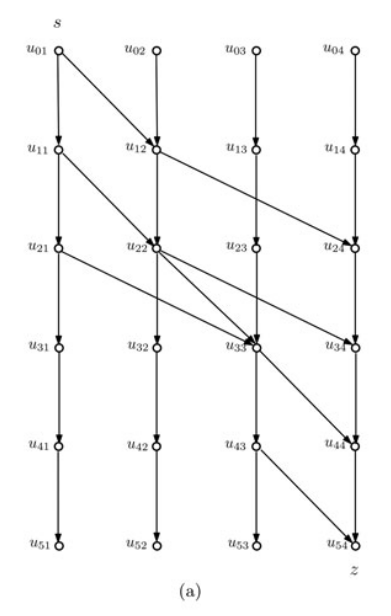
\includegraphics[height=0.8\textheight]{media/static_expansion_of_graphs.png}
	\end{center}
	\cite[page 318]{Michail2015}
\end{frame}

\begin{frame}{Static expansion of a temporal graph}
	\begin{tcolorbox}[definitionstyle, title=Definition: static expansion of a graph]
		The static expansion of a temporal graph $D = (V, A)$ with $V = \{ u_1, u_2, ..., u_n \}$ is a DAG $H = (S, E)$ with:
		$$ S = \{ u_{ij} | \lambda_{min} - 1 \leq i \leq \lambda_{max}, 1 \leq j \leq n \} $$
		and
		$$ E = \{ (u_{(i - 1)j}, u_{ij'}) | \lambda_{min} \leq i \leq \lambda_{max} \land $$
		$$ 1 \leq j, j' \leq n \land (j = j' \lor (u_j, u_{j'}) \in A(i))) \} $$
	\end{tcolorbox}
\end{frame}


\begin{frame}{Repetition - walks and paths in static graphs}
  \begin{itemize}
    \visible<2->{
      \item A \textbf{\textit{walk}} is a finite or infinite sequence of edges which joins a sequence of vertices.
    }
    \visible<3->{
      \item A \textbf{\textit{path}} is a walk where all vertices are distinct.
    }
  \end{itemize}
\end{frame}


\begin{frame}{Journeys}
	\begin{tcolorbox}[definitionstyle, title=Definition: temporal/time respecting walk]
		A \textbf{temporal} or \textbf{time-respecting walk} $W$ of a temporal graph $D = (V, A)$ is an alternating sequence of of nodes and times $(u_1 , t_1 , u_2 , t_2 , ... , u_{k-1} , t_{k-1} , u_k )$
		where 
		\begin{itemize}
			\item $\forall 1 \leq i \leq k - 1: ((u_i , u_{i+1} ), t_i ) \in A$ and
			\item $1 \leq i \leq k - 2: t_i < t_{i + 1}$
		\end{itemize}
	\end{tcolorbox}
	\begin{itemize}
		\item $t_1$ - departure time
		\item $t_{k - 1}$ arrival time
		\item $t_{k - 1} - t_1 + 1$ - duration/temporal length
	\end{itemize}
\end{frame}

\begin{frame}{Journeys}
	\begin{tcolorbox}[definitionstyle, title=Definition: Journey]
		A \textbf{journey} is a is a temporal walk with pairwise distinct nodes \^{=} a journey of D is a path of the underlying static graph of D that uses
strictly increasing edge-labels.
	\end{tcolorbox}

	\visible<2->{
    \begin{tcolorbox}[definitionstyle, title=Definition: Foremost Journey]
      A u-v journey J is called foremost from time $t \in \mathbb{N}$ if it departs after time t and its arrival time is minimized.
    \end{tcolorbox}
  }
\end{frame}

\begin{frame}{Journeys}
	\begin{tcolorbox}[definitionstyle, title=Definition: Temporal distance]
    The \textbf{temporal distance} from a node $u$ to at time $t$ to a node $v$ is defined as the duration of a foremost journey from $u$ to $v$ that departs at time $t$.
	\end{tcolorbox}
	\visible<2->{
	  \begin{tcolorbox}[definitionstyle, title=Definition: Temporal diameter $d$]
     The minimum integer $d$ such that there exists a foremost journey from every node $(u, t) \in V \times \{ 0, 1, ..., \alpha - d \}$  to every node $v \in V$ with duration at most $d$.
  	\end{tcolorbox}
  }
\end{frame}



\begin{frame}{Computing foremost journeys - Problem formulation}
  \begin{center}
    Given a source node $s \in V$ and a start time $t_{start}$ compute the foremost $s-w$ journey for all $w \in V \textbackslash{} \{ s \}$
  \end{center}
\end{frame}

\begin{frame}{Sidenote - offline vs. online algorithms}
  \begin{minipage}{0.45\textwidth}
    \underline{offline algorithms}
    \begin{center}
      takes whole temporal graph $D$ as input
    \end{center}
  \end{minipage} \hfill 
  \begin{minipage}{0.45\textwidth}
    \underline{online algorithms}
    \begin{quote}
    temporal graph is revealed to algorithm over time
    \end{quote}
  \end{minipage}
\end{frame}

\begin{frame}{Computing foremost journeys - Algorithm}

\end{frame}

\begin{frame}{Computing foremost journeys - Proof of correctness}


\end{frame}
\begin{frame}{Computing foremost journeys - Running time}

\end{frame}



\begin{frame}{The government has been lying to us}
	\begin{figure}
		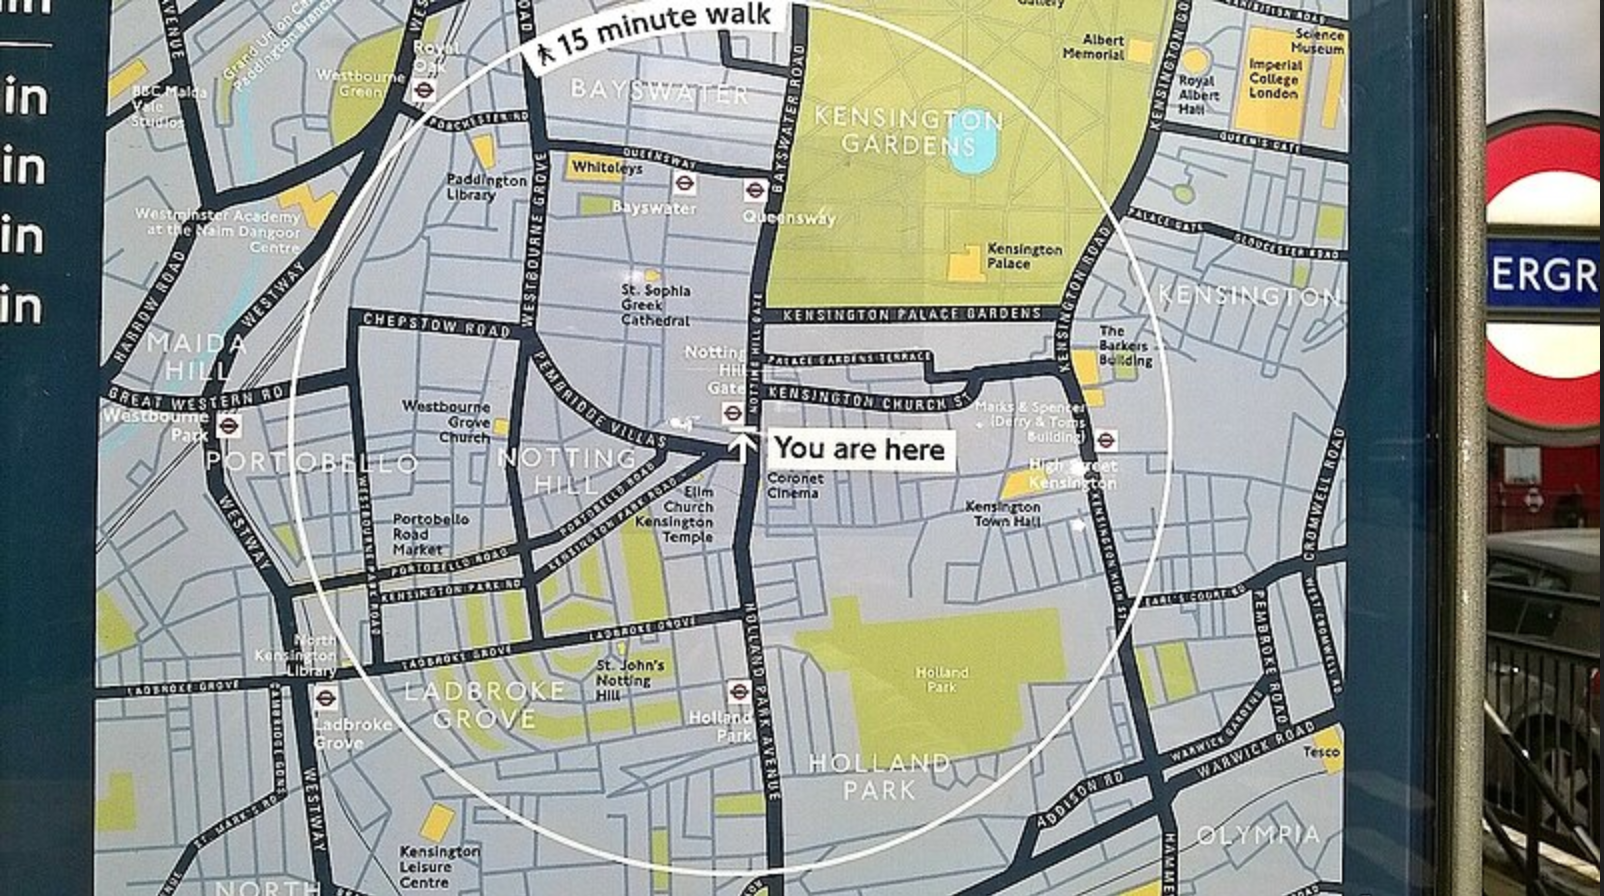
\includegraphics[width=0.9\linewidth]{media/image_1737738340.png}
		\caption{You-are-here-maps are wrong!}
	\end{figure}
	\sourcefootnote{https://commons.wikimedia.org/wiki/File:Notting_Hill_Royal_Borough_Of_K\%26C_Council_Map_Outlining_the_Official_Area_of_Notting_Hill_and_the_Surrounding_Areas_2018.jpg}
\end{frame}

\begin{frame}{15 min walk}
	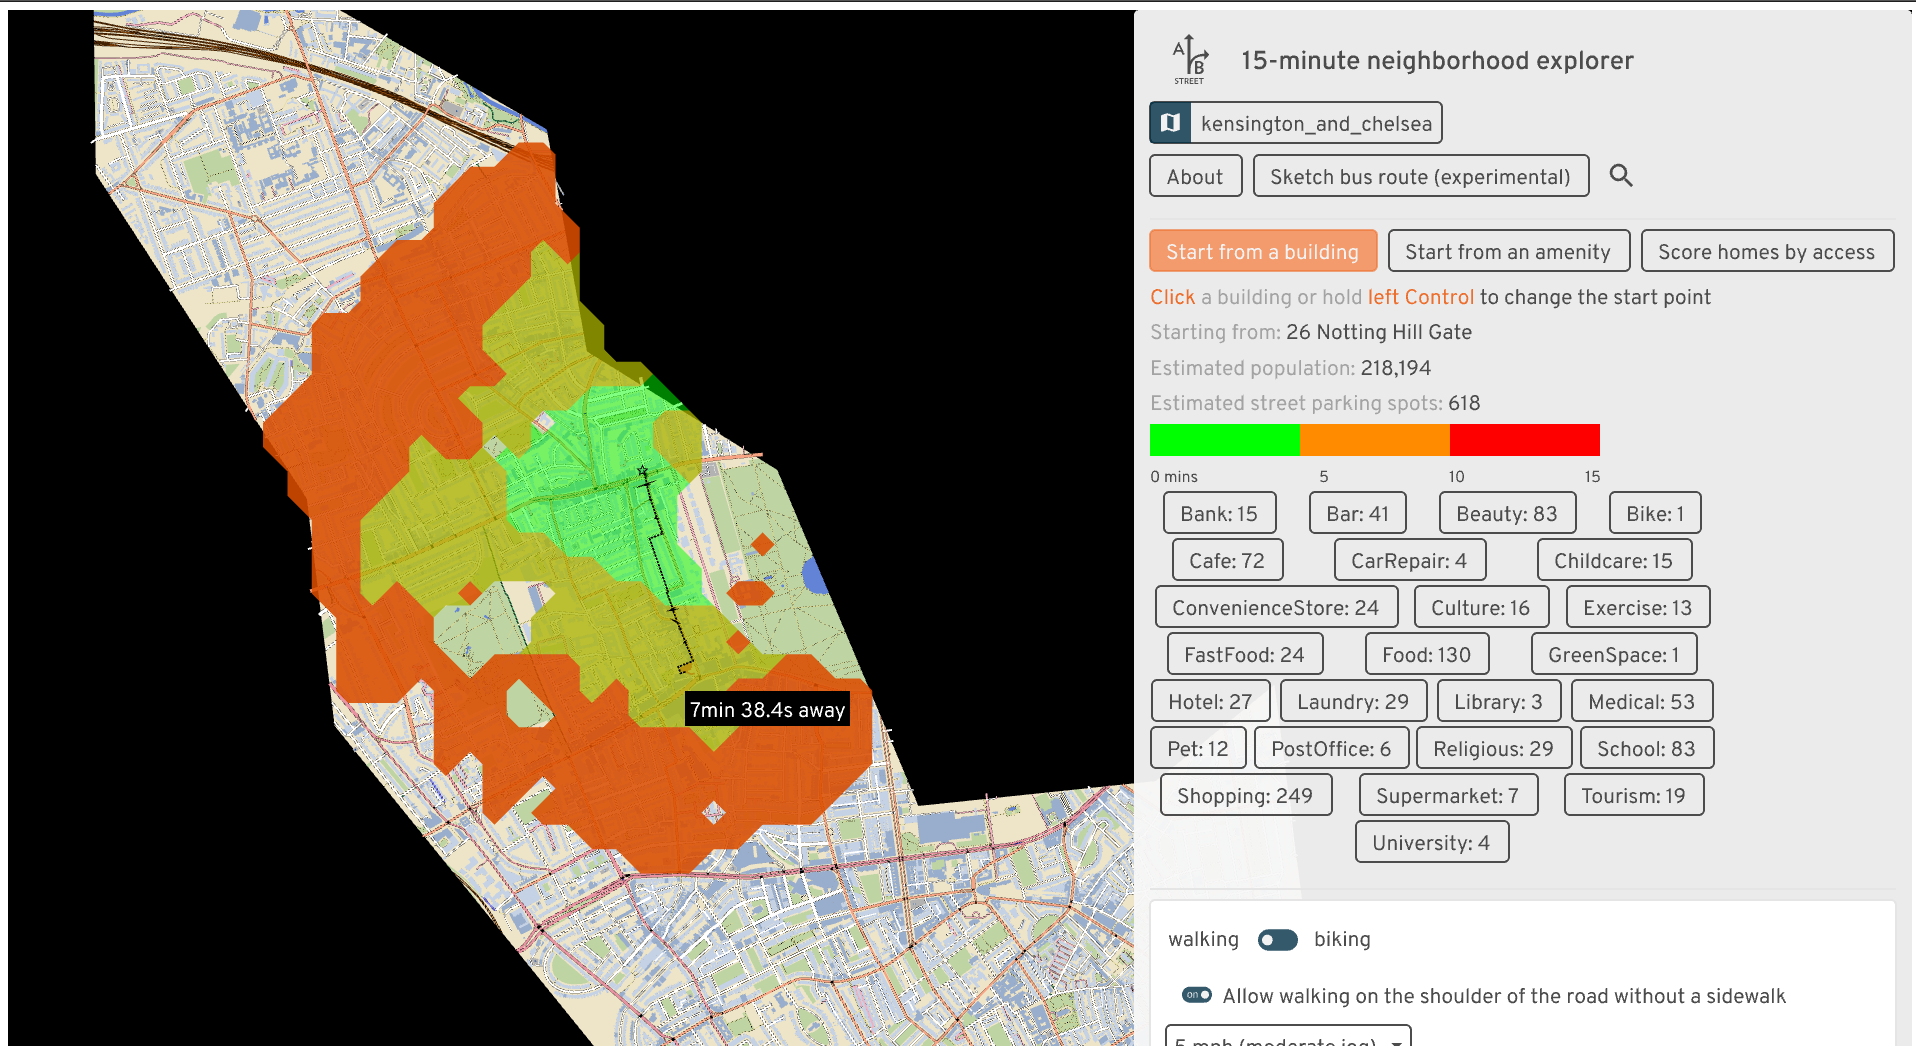
\includegraphics[width=\linewidth]{media/15-min-walk.png}
	\sourcefootnote{https://play.abstreet.org/0.3.49/fifteen_min.html}
\end{frame}

\begin{frame}{Reachability}
	\begin{tcolorbox}[definitionstyle, title=Definition: Reachability]
	\end{tcolorbox}

\end{frame}


\section{Temporal graphs for modeling dissemination processes}
\begin{frame}
  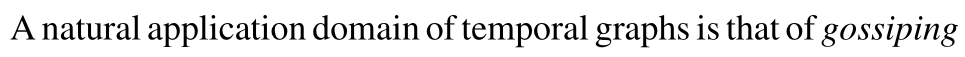
\includegraphics[width=\linewidth]{media/gossip.png} \texttildelow{} \cite{Michail2015}
\end{frame}

\begin{frame}{What are dissemination processes?}
	\begin{itemize}
		\item spread of rumors
		\item spread of fake news
		\item spread of diseases
	\end{itemize}
\end{frame}

\section{Teasers}
\begin{frame}{Temporal Graph Neural Networks}
\end{frame}

\begin{frame}{Sources}
	\printbibliography
\end{frame}

\end{document}
